\documentclass{article}

\usepackage[utf8]{inputenc}
\usepackage{graphicx}
\usepackage{geometry}   \geometry{margin=1in}
\usepackage{amsmath}
\usepackage{xcolor}
\usepackage{float}
\usepackage{longtable}
\usepackage{natbib}
\usepackage[nonumberlist]{glossaries}

\makeglossaries
\loadglsentries{glossary}


\title{Hot Swappable Pedalboard and Routing System:\\Progress Report 2}
\author{Nicholas Pham}
\date{November 2018}

\begin{document}

\maketitle
\begin{center}
    Electrical Engineering \\
    Scott Kuindersma, Jim MacAurthur
\end{center}

\newpage
\glsaddall
\printglossaries
\newpage

\section{Define}
	\subsection{Introduction}
	\color{gray}
	Many electric guitarists use effect pedals to augment their guitar amp's sound.  First developed in the 1960s, there are now thousands of pedals available for guitarists to use.  Because of the plethora of options, guitarists need an easy way to compare and interchange effects.

	In my project proposal, I proposed an integrated \emph{hot-swappable} guitar effect pedalboard and switching unit to improve the efficiency by which guitarists can change out their effects pedals to create new sounds.  The proposal focused on two main use cases: performing musicians who need to quickly change sounds, and studio musicians who need ways to radically alter their sound via new combinations of effects.

	Through discussions with my advisors, the focus of this project has shifted away from the first use model to an expanded version of the second.  Following the first step of the design process \cite{ES100Lec3}, marketing, led to this shift of focus, as there are already products available that allow performing musicians to program combinations of effects to be switched on and off at once.  Now the product will aim less to be portable and usable in real-time by a gigging musician and more useful for off-line effects swapping.  As will be further described in the next section, the product will be designed as a sales tool for retailers such as Guitar Center who sell guitar effects pedals.  By making it easier for customers to try out new combinations of pedals, this product will help retailers sell more units, and help customers discover and purchase additional processors to expand and improve their guitar systems.
	\color{black}

	\subsection{Motivation and Use Cases}

	\color{gray}
	Though in an age of Internet shopping there are many guitar related products available for purchase on-line, most players want to test potential purchases in person before buying them.  As such, brick-and-mortar music stores such as Guitar Center still have a place in the industry.
	\subsection{Testing Effects}
	The existing method for testing effects pedals at brick-and-mortar retail store such as Guitar Center is a slow process.  Once a customer requests to test a pedal, an employee brings the particular unit being test to a padded table (see Figure \ref{fig:GuitarCenterBoard}.  The employee must also find the correct power supply before connecting the unit to the guitar and the amplifier.  If a customer would like to test two pedals, for instance to decide between them which one to purchase, the employee would need to grab an additional power supply and cable for connection.  Then to perform an A-B test, the customer must turn the amplifier output off to prevent pops before disconnecting the current pedal and replacing it with the other one.  This time required for swapping the pedals limits the customer's ability to accurately judge the relative qualities of the units under test.  This cost can result in several negative consequences.  First, because of the reduction in accuracy of the A-B test, the guitarist may not be able to make a well-informed decision as to which effect best suits them, which could result in them either purchasing an inferior product, or in them deciding not to purchase any product at all.  Second, the known difficulties of testing effects pedals in this way may deter potential customers from even bothering at all, which limits the number of "impulse" purchases.  An improved method for testing guitar effects pedals at guitar stores would be beneficial to both consumers of these effects and their producers and retailers.

	\begin{figure}
		\centering
		\includegraphics[width = 0.4\textwidth]{PR2Images/GuitarCenterBoard.jpg}
		\caption{A typical "test bench" for most guitar pedals.  Guitar Center, Boston MA, September 2018.}
		\label{fig:GuitarCenterBoard}
	\end{figure}

	\subsection{Sales Displays}
	While most of the in-stock effects pedals at retailers like Guitar Center are stored in a display for customers to peruse, some larger companies have integrated displays of their products.  For example, Figure \ref{fig:BossDisplay} shows one such display, containing products from Boss, one of the most popular companies in the industry \cite{ReverbMostPopular}.  As can be seen, the pedals are permanently attached to the display board, and are connected in series with power available to all effects at once.  This solves some of the issues mentioned previously.  For pedals that are available in these displays, employees do not need to do anything for customers to test them.  Customers must only plug a guitar into an input to the display unit, which automatically connects to the first pedal.  The last pedal in the series chain is always connected to a guitar amp.

	\begin{figure}
		\centering
		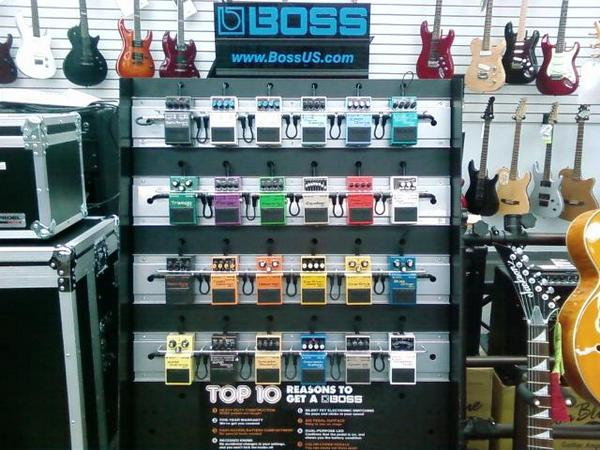
\includegraphics[width = 0.6 \textwidth]{PR2Images/BossDisplay.jpg}
		\caption{A display of Boss pedals typical to those found at retail stores such as Guitar Center \cite{BossDisplayPhoto}}
		\label{fig:BossDisplay}
	\end{figure}

	However, this system does have some limitations.  The first issue stems from the bypass method of many of these units.  Many guitar pedals, including all products offered by Boss, include a buffer that is active when the main "effect" is bypassed (see Figure \ref{fig:BufferedBypassConfig}).  This is useful for performing guitarists who often use cables totaling up to fifty feet in length.  The capacitive loading from the coaxial cable can result in high frequency loss, as guitar pickups can have DC output resistance on the order of $10k\Omega$.  A high input impedance and low output impedance buffer placed closer to the guitar can reduce the effects of this high frequency roll-off, which is typically undesirable.  However, because these display boards can contain up to thirty or more effects, there can be issues with signal degradation \cite{OrmanBypassMeasurements}.  This results in an inaccurate representation of the sound of any single pedal in the display.

	\begin{figure}
		\centering
		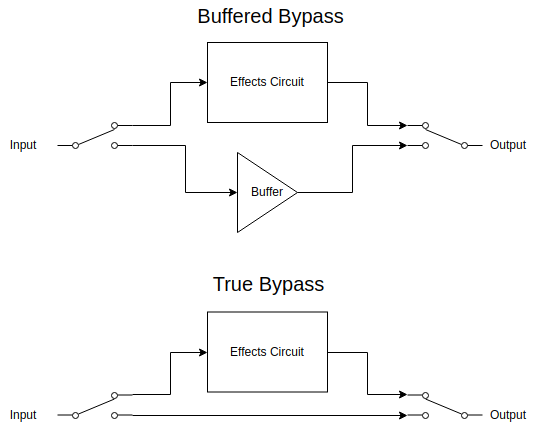
\includegraphics[width = 0.6 \textwidth]{PR2Images/BufferedvTrueBypass}
		\caption{Comparison of Buffered Bypass vs True Bypass topologies.  With the former, a buffer is in still placed in the signal even when the effect circuit is bypassed (some forms include the buffer prior to the effects circuit so the input is always buffered).  The true bypass topologies mechanically bypasses the effect circuit with a wire.}
		\label{fig:BufferedBypassConfig}
	\end{figure}


	Another issue is the fixed order and routing of the effects in the display.  The connection topologies between effects units can result in radical differences in output, which can affect the perceived quality of a pedals sound, when used in conjunction with others.  For example, consider the different topologies for connecting a distortion and delay pedal in Figure \ref{fig:PedalConnectionTopologies}.  The first one shows the guitar connected to the distortion pedal, which has its output connected to the input of a delay pedal, which in turn is connected to the guitar amplifier.  In this case, the sound might be the main distorted guitar sound with some dying echoes of the distorted sound.  The second topology shows the guitar connected to the distortion and delay pedals in parallel, which would result in the main distorted guitar sound and echoes of the "clean", unaffected guitar.  Finally, the third case shows the guitar first connected to the delay, which is them connected in series with the distortion pedal.  In this case, though the repeats of the delay decrease in amplitude over time, the non-linear clipping of the distortion pedal results in the echoes sounding at equal volume, all heavily distorted.  As can be seen even with this simple example involving only two effects, there are a multitude of possible connection topologies typically available to guitarists who own guitar pedals that are not available for testing on such display boards.

	\begin{figure}
		\centering
		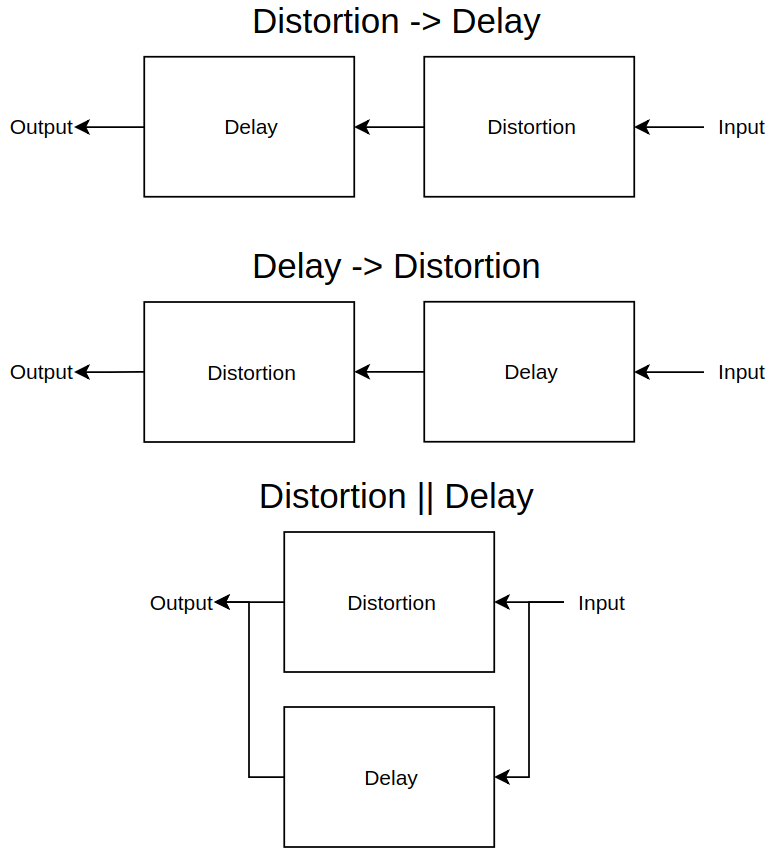
\includegraphics[width = 0.4 \textwidth]{PR2Images/RoutingConfigs.png}
		\caption{Example of the different ways to combine just two pedals.  More than two effects will have exponentially more options}
		\label{fig:PedalConnectionTopologies}
	\end{figure}

	\subsection{Studio Musicians}

	While this discussion has so far focused on guitarists as customers in a store, the same issues can face studio musicians hired for recordings.  These musicians must be able to produce any tone that their boss, the producer or artist who hired them, wants for the recording.  Because studio and musician time is very expensive, these studio musicians may have limited time to decide on and set up their equipment before recording begins.  Typically they might plug in pedals individually much as a customer does at a guitar store, which shares the issues described above.  Alternatively, some studio musicians might have their effects pedals integrated into an automatic switching system alluded to in the Overview.  However, these systems are often not intuitive to program, which means that the musician may set up a limited number of "presets", combinations of effects, that they will use.  This can limit their creativity in developing new sounds for their recordings.  A more intuitive system for connecting the effects pedals they already own would facilitate their creativity and save money by reducing the time spent on the mechanics of changing out equipment.
	\color{black}

	\subsection{Prior Art}
	\color{gray}

	In addition to the displays mentioned above, there are several patents related to this project.

		\subsubsection{Magnetic Pedal Attachment}
		The Earthboard from Rare Earth Music LLC uses a unique system of magnets both to attach pedals to the pedalboard and to provide simple power to them.  Pedals are attached on a plate via a hook and loop device such as velcro.  Then the plates magnetically attach to long metal rails.  The two rails provide 9VDC power to the pedals via cabled connections between pedal and plate \cite{EARTHBOARDSITE}.

		\subsubsection{Bracket Attachment}

		U.S. Patent Grant US9620094B2 describes an improved method for attaching pedals to a pedalboard \cite{ABBATE:2016}.  Using small brackets which are directly mounted to the pedal enclosure via the bottom cover screws, this method for mounting pedals is much more stable and solid than velcro or zip-tie methods, while also using few external materials. However, this implementation describes directly attaching the pedals to the pedalboard, which will require other screws. This means the pedal placement will be fairly permanent and it will be difficult to swap out pedals, necessitating the use of external tools such as a screwdriver.

		\subsubsection{Modular Effect System}

		U.S. Patent US4479238A describes an effect system incorporating a main parent enclosure which contains power and signal routing circuits and receiving slots for effect modules \cite{SPECTOR:1982}. These modules contain effects circuits built into a special form factor that allows them to be inserted into the slots and make signal and power connections with the main unit. The main enclosure contains routing circuits which can choose, remotely or on the front panel, which effects should be connected, much like the automatic routing systems described previously. In addition, the housing automatically bypasses any slot in which no module is fully inserted, preventing issues with ”hot-swapping”, or removing the effect card while the system is in use. This system does a nice job of allowing different combinations of effects to be tested, but it does have a significant limitation. The effect modules must be of the correct card format, which limits the user to specifically designed units. As the guitar pedal form factor is so ubiquitous (though not exactly standardized: pedals may come in many shapes and sizes), a guitarist using this system would not be able to incorporate the majority of effects units offered today, and would not be able to use any pedals they already own. In addition, because of their design, these card modules cannot be used in absence of the main enclosure unlike normal guitar pedals, further limiting their flexibility.

		\subsubsection{Waterproof Swappable Effects System}

		U.S. Patent USD782567S1 describes a pedalboard system which allows guitar effects pedals to be attached magnetically to a pedalboard \cite{FAORO:2015board}.  The system allows for hot-swappability of effects, which are connected to the board's internal routing via contacts underneath: no external cables are required.  While the patent has very little detail on the capabilities and specifications of the product, it is available for sale from Nexi Industries \cite{NexiIndustries}.  Their website claims that the switching in both the pedals and on the board is "true bypass", which in industry terminology means that the effects circuits are mechanically switched out of the signal path when bypassed, as opposed to electronic switching with buffers mentioned above.  The initial system was designed to be used specifically with proprietary effects pedals, covered in U.S. Patent USD782566S1 \cite{FAORO:2015pedal}.  However, the manufacturer has since released a product to interface with third-party guitar effects \cite{conNEXI}.

		The product does offer a solution to many issues thus far described.  In particular, it allows for fast swapping of effects pedals without the need for unplugging signal and power cables.  However, it does have some issues.  The interface between the pedal and the plate still relies on uncontrolled lengths of cable required to make connections with the pedal's input and output jacks.  The system also supposes a single power supply type, 9VDC through a 2.1 mm center negative plug.  While this is fairly standard, there are a number of popular effects, particularly more powerful digital ones, that require different power supplies.  There is also no improvement on the mechanism for attaching third party effects to the plates: the marketing examples show zip-ties being used, which can damage the pedal \cite{conNEXI}.  The pedal plates also only come in one size which is not suitable for many larger pedals.  Finally, the system supports only a single series routing option, which eliminates many possible routing topologies.

	\color{black}

	\subsection{Specifications}
	The main issue with the current system of testing guitar pedals is the inconvenience and speed of switching between different units.  The following specifications directly relate to reducing the inconvenience and time required to swap between different units when demoing.

	\begin{center}
	\renewcommand{\arraystretch}{1.5}
	\begin{tabular}{|l|l|l|p{6cm}|}
		\hline
		Metric & Min Target Value & Preferred Target & Justification \\
		\hline
		Swapping Time & 80\% reduction & 90\% & To be useful, the solution should offer a major improvement in swap time.  As current swap time is on the order of 10 seconds, the improved switching time should be on the order of 1 second.\\
		Compatibility &  $>$80\% & $>$ 95\% & In order to be an effective tool, the solution must be usable with a majority of pedals available at typical retail locations.  80\% is reasonable because a majority of retailer stock contains pedals by a handful of brands.  There is a trade-off between compatibility versus function and form, so designing for any possible pedal is not possible. \\
		Intuition & $< 250$ words& $< 150$ words & In order to quantify the ease of use and intuitiveness of using the solution, a simple metric might be number of words required to give working knowledge in a user guide.  If the solution is easy to use and intuitive, it should not take long to teach a new user how to operate it.  250 words can easily fit on a double-spaced page, and most people can speak about 150 words per minute. \\
		\hline
	\end{tabular}
	\end{center}

	After these primary specification follow several additional requirements which ensure that the solution will be useful.

	\begin{center}
	\renewcommand{\arraystretch}{1.5}
	\begin{longtable}{|l|l|l|p{6cm}|}
		\hline
		Metric & Min Target Value & Preferred Target & Justification \\
		\hline
		System Cost & \$200 & \$100 & Though the price of the solution when sold to a retailer is dependent on marketing and other factors, the cost to produce the system should be relatively low, so as to make it a viable option for use as a sales tool. \\
		Incremental Cost & \$20 & \$1 & There must also be a distinction drawn between the cost of an entire system and the cost of allowing an additional pedal to interface with the system.  Because many retail stores may stock hundreds of guitar pedals, the cost of adding a single new pedal to the system must be a small percent of that pedal's cost. \\
		Signal-to-Noise Ratio & 90dB &  120dB & The electric guitar, by virtue of its simple passive magnetic pickups can have a very high SNR, measured in non-ideal circumstances at +90 dBV.  Higher values in a controlled environment are likely.  Though many guitar pedals may have lower SNRs, it is vital the solution maintain the maximum possible dynamic range. \\
		Frequency Response & 20 - 20 kHz & DC - 30 kHz & As an audio system, the solution must at minimum pass the audio range.  Because the solution might be used with processors that could output DC voltages (such as control voltage signals), the frequency response should extend down to DC.  Ideally, the frequency response would exceed 20kHz to allow for higher frequency components generated by the guitar and nonlinear effects pedals. \\
		Switching Time & 125 ms & 20 ms & When swapping a pedal in or out of the system, there should be no perceptible delay between when the pedal is inserted and when the sound becomes effected.  125 ms is the threshold for detectability of sound latency against visuals \cite{Timing}.  An ideal target would be in the range of tens of milliseconds, below which the Precedence effect suggests that there would be little discontinuity heard \cite{PrecedenceEffect}. \\
		Transient & $<$0.5 dB & $<$ 0.1 dB & When swapping a pedal in or out of the system, any transient created must not damage connected equipment (such as the amplifier) or be disturbing. \\
		SELV compliance	& Yes & - & For ease of design and safety, the solution should accept DC voltage from an external AC/DC converter.  Through Separated Extra Low Voltage (SELV) compliance, the solution will not need to design for high voltage safety, which would reduce design and regulation/testing costs. \\
		\hline
	\end{longtable}
	\end{center}

\section{Design}
	\subsection{System Level Description}

	Though it may appear trivial at first, the broad scope of the design space of this project means making difficult design decisions where there is often no clear answer.  One of the biggest up front challenges is in developing the method to standardize the physical and electrical connections that will be used for the hot swapping feature.  

	Data collected during a site visit to a Guitar Center retail location in Boston demonstrated the plethora of effects pedals available at brick-and-mortar stores \cite{MyPedalData}.  These 150 guitar pedals represent a good mix of products, from mass market production units such as the Boss DS-1 to high quality and expensive effects like Eventide's H9.  While the major manufacturers like Boss, MXR, and Electro Harmonix have narrowed their form factors down to a handful of types each, there is no standardization across producers on features important for this project, including the dimensions of the enclosure, the location and orientation of the signal and power jacks, the location of the screws used to hold the pedal's bottom plates.  Though most products use the de facto standard 9 VDC, center negative power supply connected with a 2.1 mm plug, this too has variations in some cases \cite{MyPedalData}.  All of these variations complicate standardizing a form that can easily be hot swapped.

	\begin{figure}
		\centering
		\includegraphics[width = 0.6\textwidth]{PR2Images/GCpedals.jpg}
		\caption{Just some of the many pedals available on hand at Guitar Center, Boston MA.}
		\label{fig:GCpedalscase}
	\end{figure}

	The design process has focused on ease of use and intuition for the user over any other considerations where possible, which explains the preference for this tactile and tangible hot swapping method over some programmable switcher, as seen in \cite{ProgrammableSwitcherExample}.  This push for simplicity led to some increases in design complexity, including the need to automatically detect the hot swapping event rather than a separate user controlled switch.  The other major consideration was flexibility and a wide range of compatibility, though there were sometimes trade offs associated with supporting some less common features.

	To illustrate the main features and mechanisms of the solution, a block diagram is shown in Figure \ref{fig:SystemBlockDiagram}.  The individual blocks and their functions are summarized below.

	\begin{figure}
		\centering
		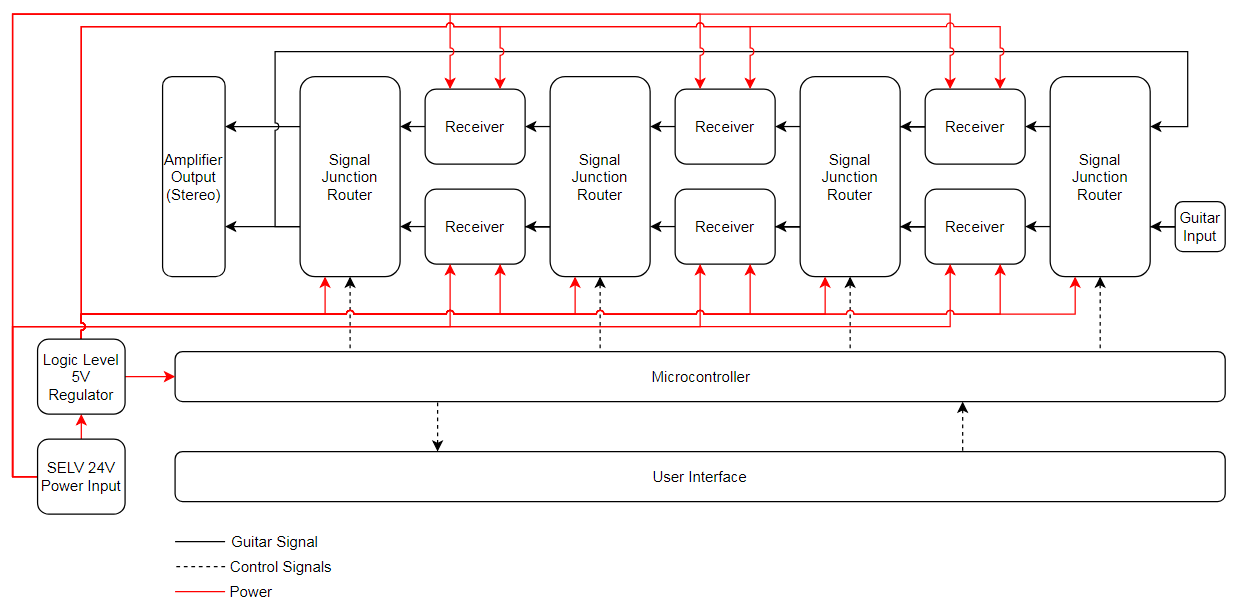
\includegraphics[width = \textwidth]{PR2Images/SystemBlockDiagram.PNG}
		\caption{Block Diagram of the Solution}
		\label{fig:SystemBlockDiagram}
	\end{figure}

	\subsubsection{Plate}
	Because of the large variety of guitar pedal shapes, they are not suitable for hot swapping in and out of a fixed receiving unit.  A simple and unobtrusive way to standardize their connections and physical form is through an interfacing plate.  To make ready for integration, a pedal will be outfitted with one of these trays on which it is mechanically attached.  The input, output, and power jacks are connected to the plate via short leads with standard plugs.  These leads can be removed and replaced to accommodate variations in plug location and size.  The plate makes these leads exposed to a standardized electrical interface for insertion into the hot swap receiver.

	\subsection{Receiver}
	A receiver is the dual of the plate.  It is a receptacle for a plate, and makes the necessary power and signal connections to allow the pedal to operate.  The receiver must also detect when a plate has been inserted or not.  When a plate is present, the receiver should send the guitar signal from its input to the plate, and return the output of the pedal coming from the plate to its output.  Otherwise, it should route the signal from its input straight to its output, bypassing the send/return loop.

	\subsection{Junction Signal Router}
	The signal routers are used to direct the outputs of certain receivers to the inputs of others to allow multiple pedals to be used at the same time.  The simplest router would be a single wire connecting the output of one receiver to the input of the next, but this limits the number of options available to make these signal connections.  The router should be as transparent to the signal as possible.

	\subsection{User Interface}
	The user can control a few functions of the product.  The primary one is the automatic bypassing of pedals when they are removed from plates.  The other major component is the communication of the current routing status and the ability of the user to control this routing.  These should strive to be as clear and intuitive as picking up the pedals.	
	
	\subsection{Design Choices}
		\subsubsection{Pedal-Plate Mounting}
		\color{gray}
			\paragraph{Through Screws}
			One important subsystem is the mounting of the pedals on their plates.  One attractive option is the use of screws through the pedal's bottom cover, as described in \cite{ABBATE:2016}.  This is the most visually simple technique, but relies on pedals that have similar screw hole locations.  As discussed below, while pedals from a single manufacturer tend to come in only a handful of form factors, the locations are not always standard across manufacturers.  In addition, some pedals do not have screws on opposite corners, which is required for a secure connection.  For instance, the Ibanez TS-9 Tubescreamer has bottom cover screws only on the upper (north) side of the pedal.  Because of this type of issue, the screw-through-plate method may not work for all pedals.  \color{black}{
			In addition, to make use of the pedal's original screws, the plate material must be thin enough to allow the screws to pass through and still firmly grasp their threads.  This is discussed and accounted for in the choice of plate material.}\color{gray}

			\paragraph{Clamp}
			Another option for attaching pedals to their plates is via a clamping mechanism.  Figure \ref{fig:CornerClamp} shows a preliminary design for such a clamp, which would be used to attach pedals with irregular bottom screws.  The bracket would be located in x-y position by the bolt hole to the corner of the pedal, and would be firmly held down in the z direction by a bolt clamping through the plate. The inner sides of the bracket should be rubber or a similar surface that will not damage the finish of the pedal. \color{black} Because the screw method is compatible with so many effects, the clamp will not be pursued in the near future.  Only if a higher compatibility is required and time permits will this clamp method be examined further. \color{gray}

			\begin{figure}
				\centering
				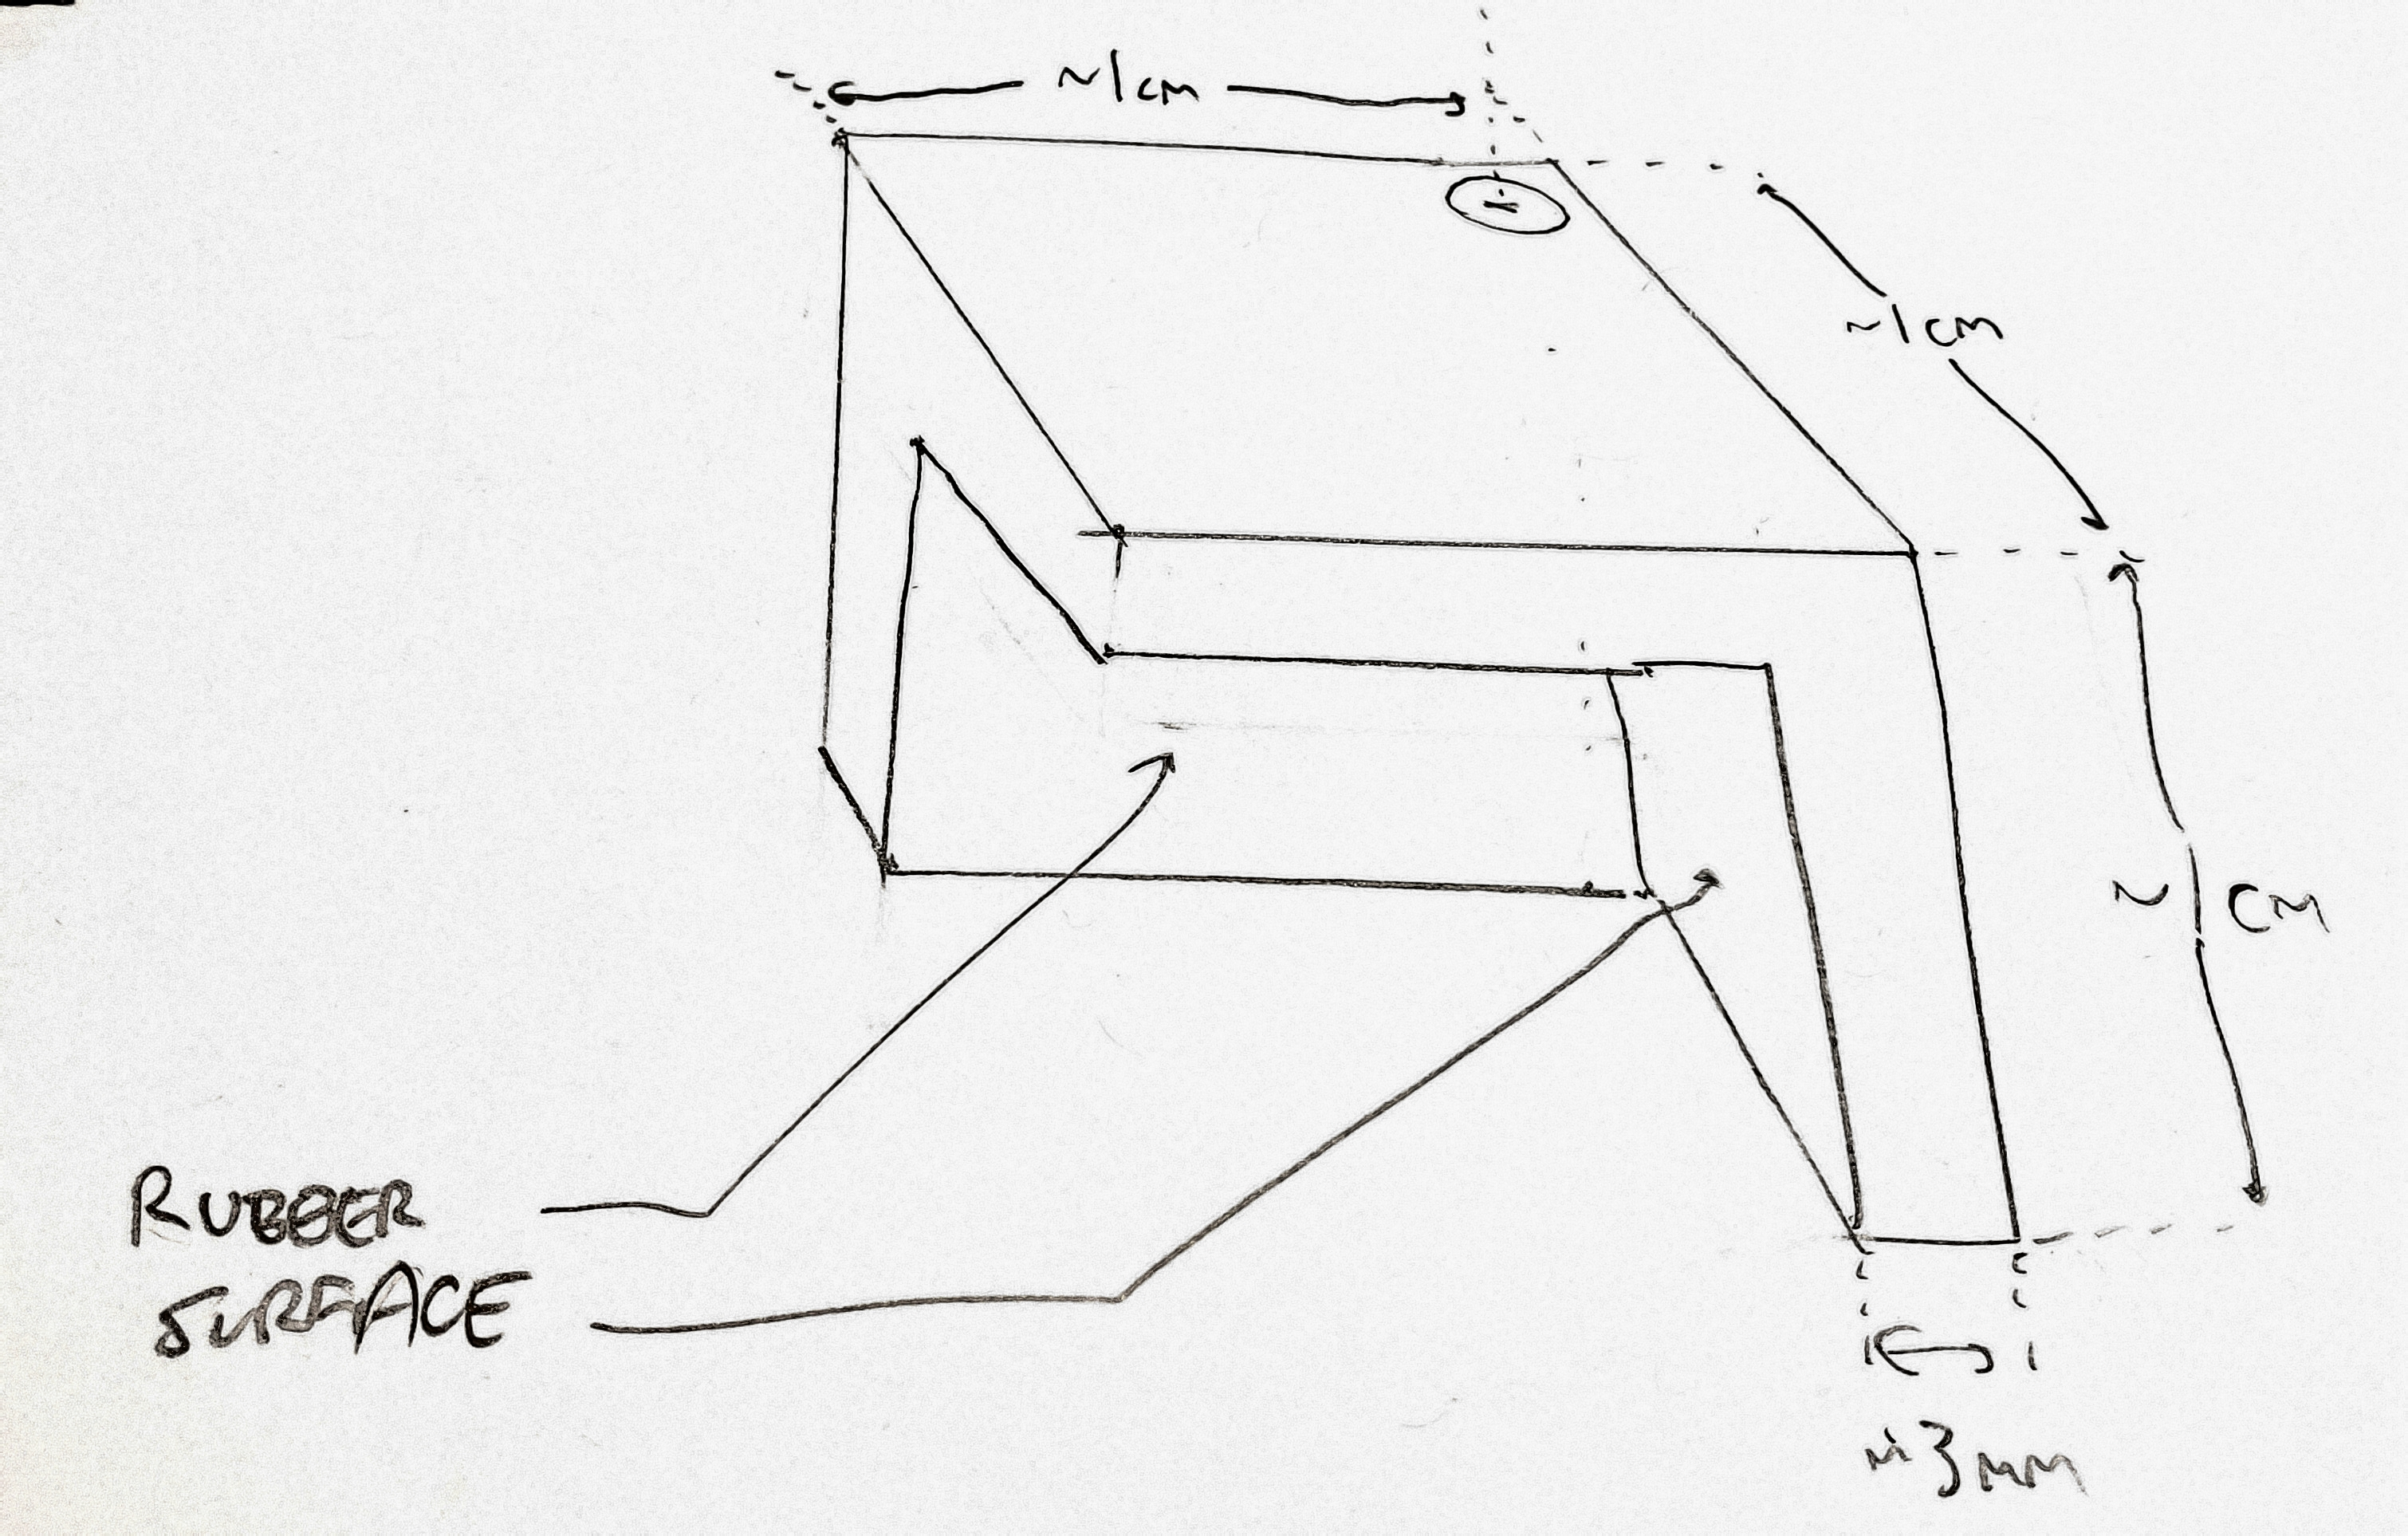
\includegraphics[width = 0.3 \textwidth]{PR2Images/CornerBracketPerspective.jpg}
				\caption{View of prospective design for corner clamp.}
				\label{fig:CornerClamp}
			\end{figure}

			\paragraph{Linear Travel}
			Because of the incongruities between effects pedals of different manufactures, a single set of bolt holes through the pedal plate will not suffice to accommodate most effects.  To solve this, the design will incorporate some combination of multiple holes in different locations and some slots through which the bolts can pass.
			\color{black}
			To develop a flexible pattern of screw slots and holes, the dimension data collected from a sample of pedals from a Guitar Center retail location \cite{MyPedalData} was plotted in MATLAB, according to the dimension of the pedals' bottom plate screw holes, as seen in Figure \ref{fig:MATLABdimdata}.  The dimensions were grouped and a best fit line drawn for the main cluster.  This line was use to design a rapid prototype plate, seen in Figure \ref{fig:PlatePrototype}.  Fabricated using a laser cuter, the plate easily accommodates several average sized pedals that were easily available for this test.  Because of this success, this method of implementation of plate-pedal mechanical interface will be pursued for the first main prototype.

			\begin{figure}
				\centering
				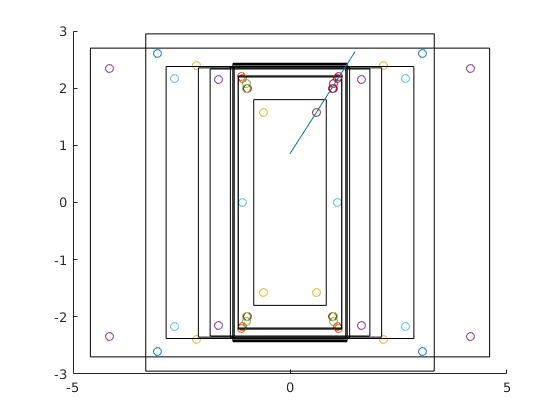
\includegraphics[width = 0.6\textwidth]{PR2Images/PedalBestFit.jpg}
				\caption{Plot of Common Guitar Pedals' Dimensions with Best Fit line through their bottom plate screw holes.}
				\label{fig:MATLABdimdata}
			\end{figure}

			\begin{figure}
				\centering
				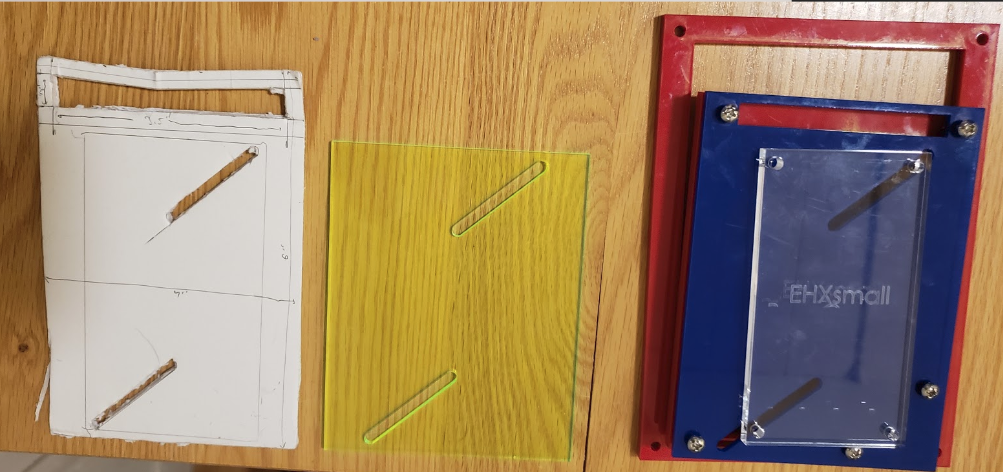
\includegraphics[width = 0.6\textwidth]{PR2Images/PlatePrototype}
				\caption{Prototypes of the pedal-plate attachment design.}
				\label{fig:PlatePrototype}
			\end{figure}

		\subsubsection{Plate Material}
		\label{Plate Material}
		The design of the plates was mainly informed by the incremental cost specification.  To keep the cost of producing a single plate low, the plate should be as simple as possible to fabricate.  As the plate requires a relatively large surface area, at minimum the size of an "average" guitar pedal, yet does not require for function significant thickness, the ideal form would be a single sheet of material.  The important design considerations for the material are that 
		\begin{itemize}
			\item the material must be rigid on the scale of a 5 x 5 inch plate.
			\item the material must be thin enough for the screws of the bottom enclosure plates to easily pass through (less than)
			\item the material must be easily cut with readily available CNC tools, namely a laser cutter or router.
			\item the material must be inexpensive.
			\item the material must not be easily bent or broken by drops or bumps.
		\end{itemize}
		The initial prototypes for the pedal-plate mounting design used 1/8" acrylic, cut with a laser cutter, because it was easily accessible.  However, acrylic can be brittle, so it is not a good choice for repeated handling by customers.  Another option was sheet aluminum, which has the benefit of being quite thin for its strength, making it easy for the pedal's screws to pass through.  A third option was to use the FR-4 grade glass epoxy resin used to make circuit boards.  In addition to being strong and lightweight, using this material allows for a simplification of the design.  Instead of sill needing to mount a circuit board to the main body of the plate, the circuit board can be the plate.  The physical layout of the screw slots can be cut at the same time as the board is shaped.  The wires to the plugs can escape directly from the surface of the board via a two position connector (such as the SWR201-NRTN-S02-SA-WH mated with a SWH201-NULN-S02-UU-WH from Sullins Connectors \cite{Sullinsdatasheet}). Other components such as switches used to select power can also be directly mounted and integrated with the board.  For its simplicity of design and manufacture, the first prototype will use this material and method for constructing the plates.

		\subsubsection{Plate-Receiver Electrical Connection Mechanism}
		\label{Pogo Pins}
		Moving signal and power between the plate and receiver is a vital task.  Though a number of guitar pedals offer processing of stereo signals, most are fully monophonic, requiring only one input and output connection.  In addition, because almost every pedal uses a single supply (non-bipolar) voltage, the simplest scheme for connecting a plate to its receiver requires only four connections: Power, Ground, Input (Send), and Output (Return).  This means that it is feasible to transfer the signal directly with individual physical connections, rather than some serial data protocol such as $\text{I}^2\text{s}$, which might be used if there were many inputs and outputs.  The use of "hard-wire" connections also keeps the signal "pure" by eliminating any unnecessary processing, which is an important consideration for marketing purposes.

		Making a consistent electric connection between the plate and receiver calls for some sort of spring loaded connector.  Unlike the connectors mentioned in Section \ref{Plate Material}, these connections are easy to break if desired, but still maintain good contact when connected.  They do not require the two surfaces to be exactly aligned, and they require only the single part to operate (instead of a matching male and female connector).  Figure \ref{fig:springloaded} shows some examples of spring loaded connectors.  On the left are connectors typically used to connect boards together within a product.  This class of spring connector is good for high pin count connections because of the large number of pins in a single unit, which are easy to manufacture cheaply.  For example, the 00-9258 type connector from AVX Corp costs \$0.77 for 8 electrodes from Digikey.  However, because these connectors are usually made for one time use when permanently assembling a product, they are not designed for repeated use.  For instance, the 00-9258 part is has a lifespan of just 50 cycles according to its datasheet \cite{AVX_00-9258_Datasheet}, which is certainly insufficient for this application.  For an order of magnitude estimate, each plate needs to be able to withstand 100 cycles per day for at least 1000 days (though the cycles/day is likely lower and the total days is likely higher).  This gives a ballpark estimate of 100,000 cycles minimum.

		\begin{figure}
			\centering
			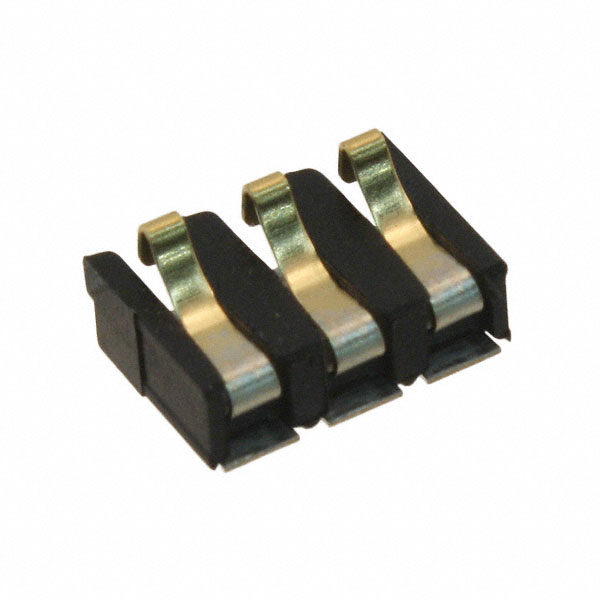
\includegraphics[width = 0.4\linewidth]{PR2Images/batteryconn}
			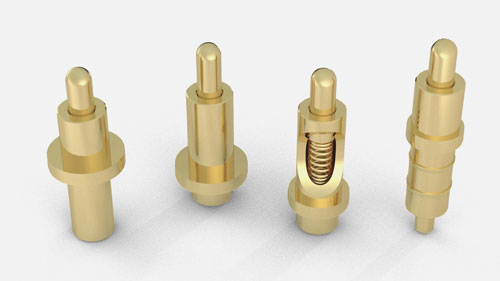
\includegraphics[width = 0.4\linewidth]{PR2Images/springpin.jpg}
			\label{fig:springloaded}
			\caption{Spring Loaded Connectors}
		\end{figure}

		In addition, because these connectors are designed for one time use, the order of connection does not matter.  However, for this application, there are some connections that must be "make-last, break-first," as will be described later.  This requires pins of different heights, which this type of multi-pin connector does not offer.  Instead, spring loaded pins like those on the right of Figure \ref{fig:springloaded} can be used.  This type of connector, sometimes known as a "Pogo Pin," includes a spring loaded plunger that sheaths into a sleeve.  These can be sourced through Digikey from Mill-Max, an industry standard manufacturer of milled connectors.  They have excellent electrical and mechanical characteristics, including 20m$\Omega$ contact resistance, minimum of 2 amp current rating, and a 1,000,000 cycle lifespan.  They come in a variety of lengths, though with less varied maximum strokes \cite{MillMax_025}.

		Using different length pins for different electrical connections allows some of these connections to be made or broken first.  In this case, most of the pins including signal and power will be of a standard height, but a shorter pin will be used to "mate-last, break-first" and will be used to ensure that the aforementioned connections are properly made before sending signal through to the plate.  In addition, a longer "mate-first, break-last" pin will be used as an inrush current limiter, as described in \cite{DesignforHotSwap}.

		Because these different pin heights are required, the design requires at least one of these spring loaded pins.  Their downside is in cost, as a pin like the costs about \$0.66 per pin.  Though the cost could be limited by using one of the multi-pin style connectors with a higher lifetime such as the Bourns 70AA series \cite{Bourns70AA_datasheet}, mixing the connection styles of the vertical-type spring loaded pins and the bending type multi-pin connectors would be difficult, in particular because of the difference in working heights.  The 0914 series spring loaded pins with the longest stroke length (for maximum height difference) are about 0.30" in height (before compression), while the uncompressed 70AA connector is 0.15" in height.  To mix these two types would require standoffs to adjust the uncompressed height, which determines the mate-order of the pins.  For simplicity, this prototype will use only pins from the 0914 series.

		Mill-Max offers many styles of spring loaded pins.  The first consideration was durability.  Though all of the pins examined are rated for 1,000,000 cycles \cite{MillMax_023}\cite{MillMax_025}, the through-hole versions likely offer better mechanical connection and stability with the circuit board, so these were preferred.  The next consideration was the ability to perform the mate-last, break-first operation, which requires as large a height differential as possible.  A large height differential will increase the time between the first and last pins making the connection, ensuring that the connections have been properly made and giving the circuit time to reach a steady state.  The pins are offered in short, standard, and long stroke lengths, which have maximum stroke depths of 0.039", 0.055", and 0.090" respectively. To achieve the longest time difference, the long stroke pins, series 0914 seem ideal.

		\begin{figure}
			\centering
			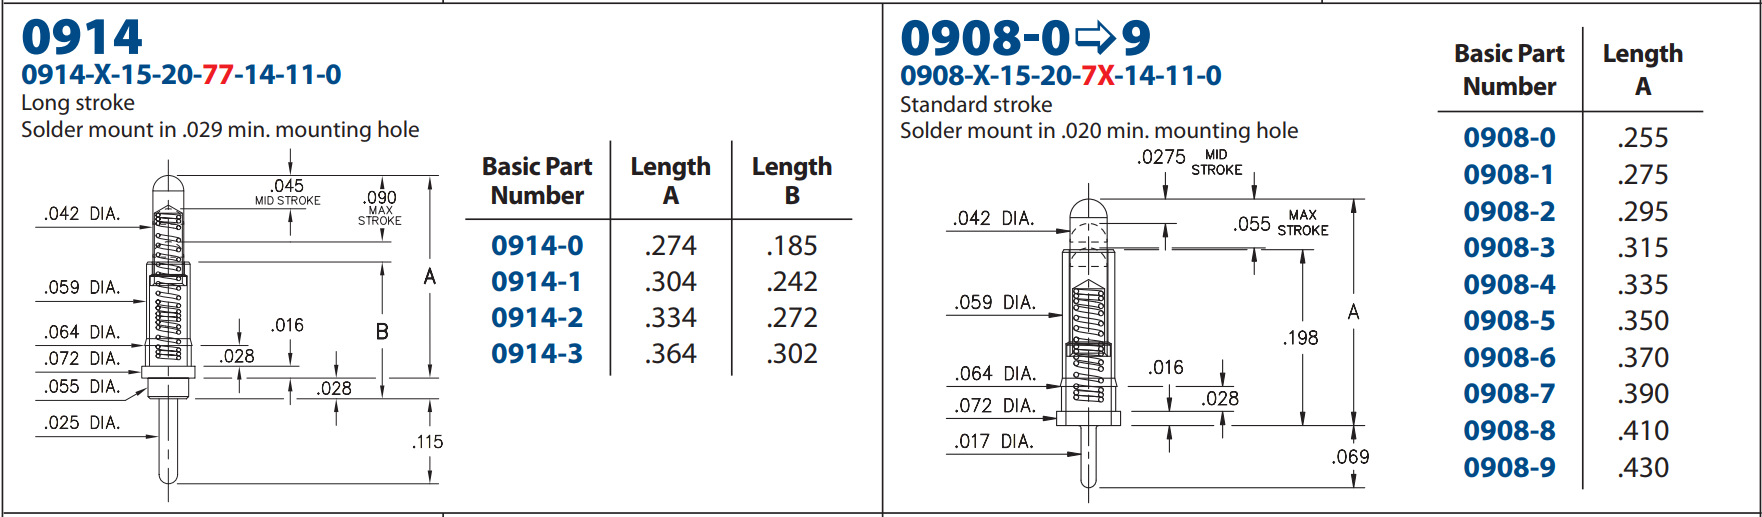
\includegraphics[width = \textwidth]{PR2Images/MillMaxSeries0914_0908.png}
			\caption{Mill Max Spring Pins, Through Hole, Long and Short Stroke}
			\label{fig:millmax0914_0908}
		\end{figure}

		As can be seen on the left in Figure \ref{fig:millmax0914_0908}, the B distance of the tallest pin determines the maximum travel of all of the pins, as this is the closest the plate can be to the surface of the receiver circuit board.  This means that 0914-0 and 0914-3 cannot be used together, as $B_3 = 0.302 == A_0 + 0.028 = 0.302$.  Only at 0914-3's maximum compression would 0914-0 make contact, so this will not work once the $\pm 0.006$ tolerances are taken into account.  However, any three consecutive pins will work together, which means choosing between using the 0914-0 and the 0914-3 (0914-1 and 0914-2 will be used in either case).  It turns out that the differences in length A any adjacent pins is 0.030", so the functional height difference between these two sets ({0, 1, 2} and {1, 2, 3}) are the same.  To reduce horizontal stress on the mounting, the shorter of the two options was chosen, as any tangential force on the end of the pin will result in less torque at the solder mount.  Thus the 0914-0 will be used for the make-last break first pins, the 0914-1 will be used for the standard input, output, and power pins, and the 0914-2 will be used for the inrush current limiting pin.

		\subsubsection{Plate Power Selection Method}
		In order to maximize the compatibility metric, the solution should be able to supply the most commonly required voltage and current supplies.  Though 9VDC is the de facto standard voltage supply \cite{MyPedalData}, there are a number of effects that accept 12 or 18 VDC, which can allow their amplifiers to have a higher headroom.  There are some other less common power supplies, such as 24 VDC for some older Electro Harmonix products, or 9 VAC for pedals like the Line 6 DL4 \cite{Line6DL4manual}, but these are rarer, so this prototype will focus on just the 9, 12, and 18 VDC supplies.

		In addition to varying electrical requirements, some pedals do not use the standard 2.1 mm power jack, with the center connector wired negative; a common alternative is a 2.5 mm jack with center positive connection.  Though this first prototype will focus on providing just the standard 2.1 mm center negative power, an extension to alternative connectors can be easily added via additional power supply cables which can plug into the plate via the same SWH201-NULN-S02-UU-WH type connector mentioned in Section \ref{Plate Material}.

		In order to supply power to the plate, there were two schemes to consider.  The first was a parallel supply, where all three voltages are connected to the plate at once, and the user who sets up the plate for a particular pedal can choose which connector to attach the power connector to.  This would allow a single voltage regulator for each supply voltage to be used.  However, this could run into issues of current draw, where many pedals could potentially draw more current than the voltage regulator can handle.  In addition, this would mean long traces in the main board carrying this voltage, which might experience a voltage drop due to the resistance of these traces.  Finally, this scheme requires two pogo pins per available voltage, one for the make-first inrush current limiting and another for the normal power supply.  Figure \ref{fig:parallelpowerschematic} shows an implementation of such a scheme.

		\begin{figure}
			\centering
			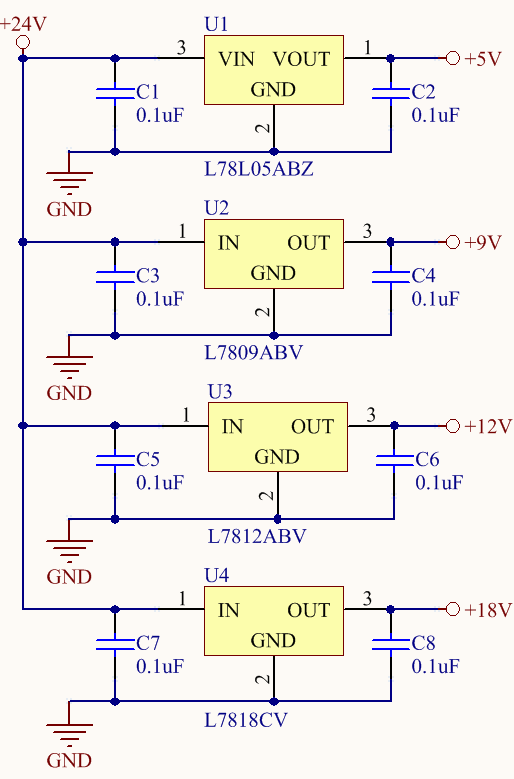
\includegraphics[width = 0.4\textwidth]{PR2Images/ParallelPowerSchematic.PNG}
			\caption{Power supply implementation where all voltages are available at all times.}
			\label{fig:parallelpowerschematic}
		\end{figure}

		The other option was to use a single voltage regulator for each plate, with a controllable output.  This eliminates concern over voltage drops between different receivers, and allows each receiver to draw as much current as a single regulator can supply.  For more than two power outputs, this method saves pogo pins, as only two pins are needed to supply the power (in addition to ground), though it does require several pins to communicate which voltage is desired for the current plate.  Instead of multiple connectors to allow the user to select the power connection, this method would use some switch, such as a two position DIP switch, to allow the user to set a binary value which can be decoded on the receiving end into the proper signals needed to control the adjustable voltage regulator.  As the pogo pins are fairly expensive (about \$0.66 each), reducing the number of pins is a good way to save on cost.

		The LM317 is a canonical adjustable voltage regulator, with its level set via a voltage divider (see datasheet section 8.2 for a typical application and design requirements \cite{LM317datasheet}).  The LM317 takes an input voltage between 1.25 and 37 V, preferably with $V_I - V_O > $ 3 V.  The difference $V_{OUT} - V_{ADJUST}$ is then kept at 1.25 V with a feedback circuit.  As shown in Figure \ref{fig:LM317_typicalapp}, this 1.25 V reference and $R_1$ then set the current through variable resistor $R_2$ ($I_{Adj}$ is negligible) which controls the output.  The $240 \Omega$ value for $R_1$ is a recommended value required to keep the output current high enough (over 3.5 mA) for a well regulated output.  The other diodes and capacitors are used to reduce ripple in the output.  Thus, $V_O$ can be given by

		\begin{align}
			V_O &= V_{REF}(1 + \frac{R_2}{R_1}) + I_{ADJ}R_2 \\
			&= 1.25 (1 + \frac{R_2}{240}) \quad \text{and} \\
			R_2 &= 240 \left( \frac{V_O}{1.25} - 1 \right) \\
			\label{eqn:LM317_R2}
		\end{align}

		However, a variable resistor for $R_2$ is not an easy method of setting the proper voltage for a user, because this would require individual tuning for each plate.  Instead, a set of switches is an easy mechanism for a user, who just needs to set the correct orientation of the switches.  A straightforward technique to use is switch in and out some additional resistors in parallel to a fixed $R_2$, as shown in Figure \ref{fig:adjustableregulatorschematic}.  Adding resistors in parallel reduces the effective resistance, reducing the output voltage, so the fixed $R_2$ should be calculated to set the maximum required output voltage, 18 VDC.  Using Equation \ref{eqn:LM317_R2} to calculate $R_2$ for an 18 V output gives $R_2 = 3.2 k\Omega$. The current through $R_1$ and consequently $R_2$ is $i_{R_1} = 1.25/240 = 5.2$ mA.  

		\begin{figure}
			\centering
			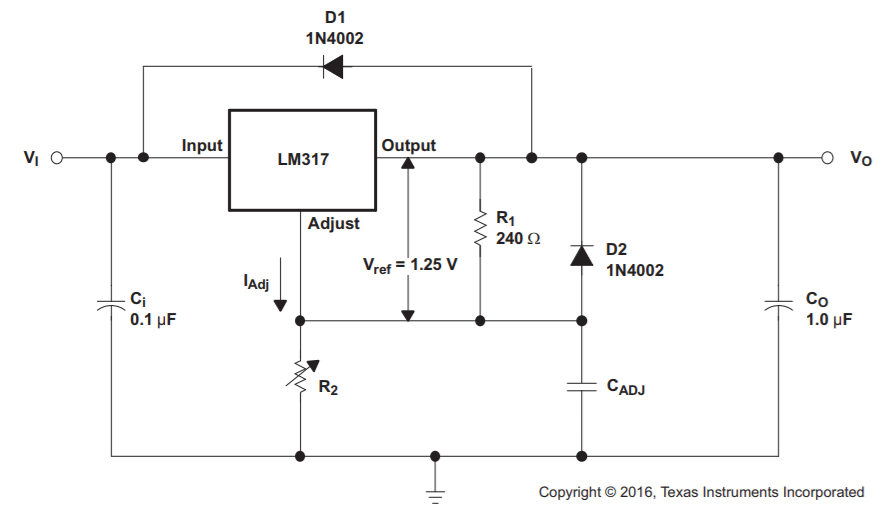
\includegraphics[width = 0.8\textwidth]{PR2Images/LM317_typicalapplication}
			\caption{Typical Application of LM317, from datasheet.}
			\label{fig:LM317_typicalapp}
		\end{figure}

		\begin{figure}
			\centering
			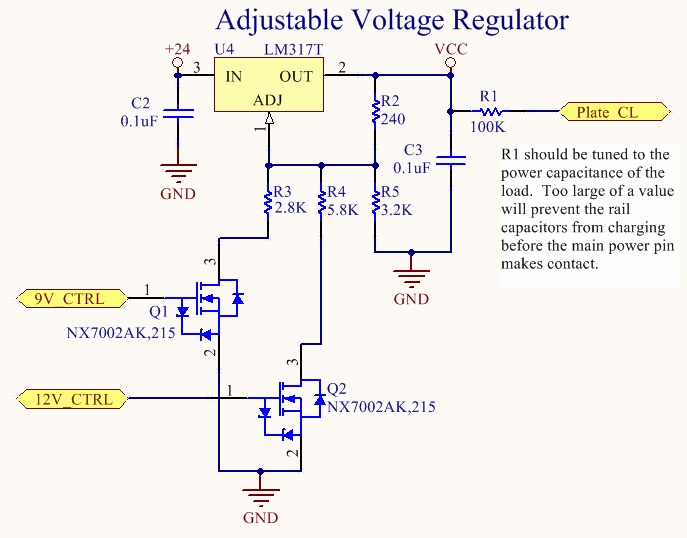
\includegraphics[width = 0.8\textwidth]{PR2Images/AdjustableRegulatorSchematic}
			\caption{MOSFET controlled adjustable regulator, with 9, 12, and 18 VDC selectable output.}
			\label{fig:adjustableregulatorschematic}
		\end{figure}

		MOSFETs are a good choice for this switch application because of their relatively low on-resistance $R_{DSon}$.  The cheapest type of MOSFET available from Digikey was the NX7002AK type, a ubiquitous single N-channel device \cite{NX7002AKdatasheet}.  With a maximum $V_{DS}$ of 60 V, a maximum $I_D$ of 190 mA for $V_{GS} = 10$ V at $25^o$ C, and a typical $R_{DSon}$ of $3.7 \Omega$ at $V_{GS}$ = 5V, this will work fine for this application, as would many standard MOSFETs.  In fact, because $R_{DSon}$ is on the order of Ohms while $R_2$ is on the order of Kiloohms, it can be neglected in the calculations for $R_3$ and $R_4$.

		For simplicity, let assume the MOSFET gate signals will not be turned on together, and that Q3 is used for a 9 V output while Q4 is used for a 12 V output, as in the following truth table:

		\begin{center}
		\begin{tabular}{c c|c}
			Q3 & Q4 & Output Voltage (V) \\
			\hline
			0 & 0 & 18 \\
			0 & 1 & 12 \\
			1 & 0 & 9 \\
			1 & 1 & X
		\end{tabular}
		\end{center}

		Because the MOSFET's on resistance can be ignored, solving for the $R_3$ when $Q_3$ is turned on so $R_3$ and $R_2$ are connected in parallel to ground gives

		\begin{align}
			R_3 || R_2 &= R_1 \left( \frac{V_O}{1.25} - 1 \right) = 240 \left( \frac{9}{1.25} - 1 \right) = 1488 \\
			R_3 &= \frac{1}{\frac{1}{R_3 || R_2} - \frac{1}{R_2}} = \frac{1}{\frac{1}{1488} - \frac{1}{3200}} = 2.8 k\Omega
		\end{align}

		Likewise, 

		\begin{align}
			R_4 || R_2 &= R_1 \left( \frac{V_O}{1.25} - 1 \right) = 240 \left( \frac{12}{1.25} - 1 \right) = 2064 \\
			R_4 &= \frac{1}{\frac{1}{R_4 || R_2} - \frac{1}{R_2}} = \frac{1}{\frac{1}{2064} - \frac{1}{3200}} = 5.8 k\Omega
		\end{align}

		Compute the power dissipated across these resistors to determine their necessary ratings.

		\begin{center}
		\begin{tabular}{c c|c}
			R ($k\Omega$) & V (V) & P (mW) \\
			\hline
			$R_1$ = 0.240 & 1.25 & 6.51 \\
			$R_2$ = 3.2 & 18 - 1.25 = 16.75 & 87.68 \\
			$R_3$ = 2.8 & 12 - 1.25 = 10.75 & 41.27 \\
			$R_4$ = 5.8 & 9 - 1.25 = 7.75 & 10.36
		\end{tabular}
		\end{center}

		Even with a 10\% safety margin, these resistors can all be 1/10 watt.

		\subsubsection{Receiver Plate-Removal Detection Method}
		To perform the automatic bypassing feature, the receiver must detect whether or not a plate has been inserted. Intuitively, the best way to do this seemed to be to use some of the same type of electrodes used to make connection between the plate and the receiver for signal and power.  This can be accomplished by using this extra detection pin as an SPST switch: when no plate is inserted, the switch is open, and when a plate is inserted, the switch closes.  This can signal some logic circuitry to activate the relay.

		To reduce transients that could result from suddenly connecting a plate and allowing the signal to flow before all of the necessary connections (Power, Ground, Input, and Output) are made, the receiver should wait to switch the relay from bypass to active until it is confident that all of the pins have made their connections.  This delay first relies on the bounce times of the pogo pins; like any mechanical switch, they will likely have some bounces or other irregularities in their switching, and one learning goal of the first prototype is to characterize this bounce.  To give an improved signal, the pin used to make this detection SPST switch will be set to "make-last, break-first," which will ensure that the other pins have already made first contact with the plate.  This is reflected in the choice of spring loaded pins described in section \ref{Pogo Pins}.  Assuming a 2 ft/s rate of descent (a high estimate) and the difference in height between the main signal connection pins and this make-last/break-first detection pin, there will be a $(0.030 in)/(24 in/s) = 1.33 ms$ difference.  Though this is likely not enough time to ensure the pogo-pins have stopped bouncing, the debouncing circuit block can and will increase this time delay before the signal to switch the relay is sent.  This time delay will need to be tuned to the specific bounce time of the pogo pins.

		To further ensure that the detect pin is the last to make contact, a second instance should be added for robustness against plates that are not inserted exactly vertically.  Assuming that the electrodes are aligned linearly, placing one detect electrode on each end of the line will ensure that both cannot make contact with the plate before the rest of the pins.  Thus, only when both electrodes have made contact should the relay be triggered.  Conversely, the relay should reset to bypass the plate when either of the electrodes break their connections.  This can be written as a boolean equation, where $A$ and $B$ are the status of the two detect electrodes (0 is disconnected, 1 is connected), and $R$ is the status of the relay, where 0 is plate-bypass and 1 is plate-active:

		\begin{align}
			R = A \cdot B
		\end{align}

		To reduce the number of pogo pins needed for this detection method, these detect pins will connect to ground, rather than 5 V, eliminating the need for an additional 5 V electrode to the plate.  Thus, these logic inputs will be active low: when a plate is inserted, the output of the switch will be 0 V, and when the plate is removed the output will be pulled up to 5 V via a pullup resistor on the receiver, shown in Figure \ref{fig:PlateDetectSwitch}.  Because of this, the A and B signals are given as their complements, and a NOR gate should be used instead of an AND.  

		\begin{figure}
			\centering
			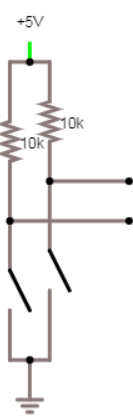
\includegraphics[width = 0.1 \textwidth]{PR2Images/PlateDetectSwitch}
			\caption{The spring loaded pins act as an SPST switch.  To reduce the necessary pins, they will connect the circuit to ground when the plate is in contact with the receiver, otherwise the pullup resistors will keep the signal high.}
			\label{fig:PlateDetectSwitch}
		\end{figure}

		On the insert transition the limiting factor on switching time (from bypassed to active) is on the order of 100 ms, the detectability threshold for visual-sound delay \cite{Timing}, which should not pose an issue with the switch debounce, logic, and relay switch times (~20 ms + ~0.1 ms + 2 ms = 22 ms \cite{EA2datasheet}).  However, the removal transition is limited by the time between the first detect electrode losing contact and the signal or power pins losing contact, which could cause transients in the output if the plate has not yet been bypassed.  By eliminating the switch debounce mechanism for this transition, the switch time can be lowered to approximately the operate time of the relay, which is about 2 ms.  This is quite close to the 1.33 ms estimate of the available window between the detect pin and the signal/power pins disconnecting.  As the estimate for this time difference is based on an order of magnitude type approximation, it is possible that there will be no issue, and no mitigation techniques need to be added.  A simple mitigation would be some transistor to pull the output to ground quickly (before the relay can be activated) so that any transients would be muted until the relay can successfully switch.  Because this would add complexity if not needed, this first prototype will proceed without this feature.

		\subsubsection{Receiver Bypass Mechanism}
		The primary function of the entire solution is to automatically bypass any receivers that do not currently have a plate inserted, so the choice of switching element is a key part of the design.  The basic choice here was between solid state analog switches or electromechanical relays.  The major design considerations for this choice are the signal to noise ratio, and the frequency response of the switching element.

		\color{gray}
		The initial value expected for the signal to noise ratio for an electric guitar was near 120 dBV.  Guitar pickups convert the mechanical energy of the vibrating strings to electrical energy via a coil of wire.  When the string vibrates in the magnetic field of a permanent magnet situated underneath, current is induced in the coil.  In an ideal environment, there should be little source of self noise because of the passive simplicity of this device, so any noise in the guitar signal is a result of the environment.  As such, the signal to noise ratio of a guitar can vary significantly based on the guitar's environment.  For example, guitar pickups are well known for their susceptibility to 60Hz line noise.  Therefore, the measured 90dBV signal to noise ratio should be taken as a minimum value, with 100dBV or more preferable.

		While solid state switches are more size, cost, and power efficient than mechanical relays, they may not have adequate signal to noise specifications, as well as crosstalk between channels on the same chip.  For example,the MT8808 Analog Switch Array \cite{Zarlink:MT8808} lists no specification on the device's signal to noise ratio, though it does boast a reasonable -90dB crosstalk between any channels for a 10kHz input with a $600 \Omega$ load.  The feed-through when a channel is off is listed as -95dB though, which is does not far exceed the minimum measured value for guitar signal to noise ratio, which could be an issue.  On the other hand, relay bypassing utilizing mechanical switches has no issues with signal to noise ratio, which would make it suitable for use in this project.

		As a minimum, the system should accommodate signals across the full range of human hearing, which is typically noted as 20Hz - 20kHz.  While this is the minimum acceptable range, there should also be allowance for lower and higher frequencies, which when used as input to a distortion effect can create inter-modulation distortion with frequencies in the audio range.  Neither of these ranges will be an issue however.  In the case that switching is accomplished with a solid state device, these are designed for frequency responses up to the tens of MHz range (the MT8808 has a 3dB frequency response of 45MHz), which is far greater than required.  If mechanical relays are used, there will likewise be no issues with frequency response in the audio range.
		
		\color{black}

		These considerations suggest a preference for using mechanical relays despite their costs.  An additional reason is some of the interactions between the circuits on the guitar and in the first engaged pedal.  As mentioned above, the guitar pickup is made from a coil of wire, typically about 42 AWG with thousands of turns around a 6 inch or so circumference bobbin \cite{StewMacpickups}.  This long thin wire produces a DC resistance on the order of $10k\Omega$, which itself is quite a high output impedance, and the inductance and some parasitic capacitances from within the pickup will result in a frequency dependent output impedance with the potential to interact with a connected circuit block with sufficiently low input impedance.  In addition, the position of the guitar's volume potentiometer can affect the output impedance (see Figure \ref{fig:guitarpickupmodel} for a model of a guitar pickup and volume control circuit).  There are a number of guitar pedals known for their interaction with the guitar's volume knob; one of the best known is the Fuzz Face, first released in 1966 by Arbitrer Electronics \cite{FuzzFace}.  Following the same calculations as \cite{FuzzFace}, the input impedance to this pedal is about $8k\Omega$.  This does not follow the rule of thumb suggesting the input impedance should be an order of magnitude greater than the output impedance of the previous circuit stage, which means that there will be interactions between the guitar and this pedal.

		\begin{figure}
			\centering
			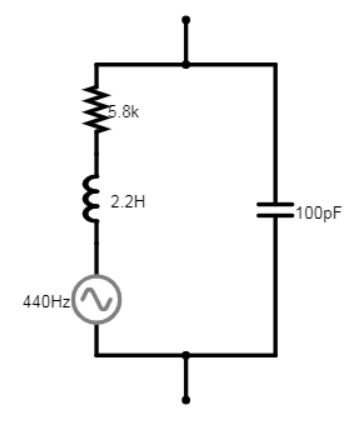
\includegraphics[width = 0.3\textwidth]{PR2Images/GuitarPickupModel}
			\caption{Model of guitar circuit.  These values are highly dependent on the particular pickups.  The potentiometer is either 250k or 500k.}
			\label{fig:guitarpickupmodel}
		\end{figure}

		Whether or not these interactions are good or bad, they have an undeniable effect on the sound and feel of playing the guitar through this pedal.  Inserting a buffer, including a solid state switch, between these circuit elements would destroy this interaction, and thus would prevent the solution from being an effect tool for comparing different pedals.  Therefore, the signal path should pass through no buffers when all receivers are bypassed, and electromechanical relays should be used to perform the switching.

		Because all of the signals being switched are low power, the relay can be in the "Low Signal Relays" category.  The cheapest available relay from Mouser was the EC2-12NJ from Kemet, a 12 V, 2 A, non-latching DPDT switch for \$1.69 each.  The DPDT type switch is preferable because only one package is required to perform the bypass switching per receiver.  The 12 V coil voltage requires less current (11 mA) than the 5 V coil which is also readily available (28 mA) \cite{EC2datasheet}.  The non-latching control makes for a very simple control circuit.  One issue with this though is that whenever the relay is activated, there is a constant 140 mW power dissipation required.  Though power is not a top priority, it would be beneficial to save power where possible, so a latching relay would be preferable in this aspect.  In addition, the datasheet claims that organic gases can build up inside the relay if the coil temperature rises due to long periods of activation current, which can result in faulty contacts \cite{EA2datasheet}, which could be solved through the use of a latching relay.  The EA2-5SNJ is available for just 9 cents more, and features a 5 V coil.  Although the lower voltage coil will draw more current when it is on, the relay needs be turned on only when being switched, so there is an overall savings in this regard.

		The EA2-5SNJ is a Form C type relay, which means that the DPDT switch operates break-before-make, ideal for this type of audio switching.  The device is a single-coil latch, where the coil is energized in one polarity to set the switch to one position, and is energized in the opposite polarity to set the switch to the other position.  This calls for an H-bridge style driver.

		\begin{figure}
			\centering
			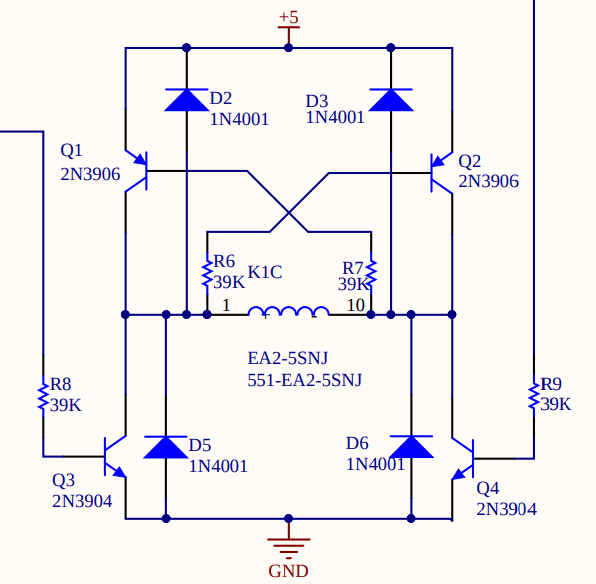
\includegraphics[width = 0.6\textwidth]{PR2Images/DiscreteHBridge.png}
			\caption{Discrete H Bridge implementation.  The inductor coil K1C load is the relay coil.}
			\label{fig:DiscreteHBridge}
		\end{figure}

		A standard discrete H bridge like the one shown in Figure \ref{fig:DiscreteHBridge} uses a quartet of transistors to power a load in either polarity or not at all.  When the two transistors in opposite corners (such as Q1 and Q4) are turned on at the same time, current flows through these transistors and the load, in this case the latching relay coil.  When it is time to set the relay's switch to the opposite position, the other two transistors are turned on instead and the load is energized with opposite polarity.  This implementation features garden-variety 3904/3906 type BJTs, which can supply plenty of current for the relay coil (just $5V/250\Omega = 20 mA$) \cite{EA2datasheet}\cite{2N3904datasheet}\cite{2N3906datasheet}, though these many other transistors would work.  D1-D4 are flyback diodes for the inductive relay coil.  To provide a load current of 

		\begin{align}
			i_{load} &= \frac{5V - V_{CE_4} - V_{CE_1}}{250 \Omega} = 18.4 mA
		\end{align}

		the base current of the transistors is related to the collector current by

		\begin{align}
			I_B &= \frac{I_C}{\beta}
		\end{align}

		The 2N3904 has a $\beta$ between 100 and 300 for a 10 mA $I_C$, so assuming $\beta = 200$ gives a required base current of

		\begin{align}
			I_B &= \frac{18.4mA}{200} = 92 \mu A \quad \text{and} \\
			R_2 &= 4.3V/92\mu A = 43 k\Omega
		\end{align}

		For a 10\% tolerance, use a $39k\Omega$ to ensure the transistor is turned fully on.

		A major issue with the H-bridge design is that both sets of transistors can never be turned on at the same time.  This would create a low impedance path from power to ground, cause high currents and potential damage to the circuit.  Though more of an issue in PWM motor control, a common application of the H-bridge, this "shoot-through" can occur when one set of transistors is switched on just as the other set is switched off.  Special protection should be taken to prevent such issues.

		For this reason, dedicated H-bridge driver ICs are offered.  One canonical example is the L298 dual H-bridge driver \cite{L298datasheet}.  It includes protection logic to prevent shoot-through and has enable inputs for each bridge.  This would be a good choice of driver, but for the price, which is about \$5 per chip from Digikey, which is more than the cost of the two relays it would be driving.  This is especially striking when considering that the cost of the MMBT3904 and MMBT3906 are \$0.10 and \$0.13 each.  For an integrated solution to be viable, it should not cost more than the relays it is driving.  Other options are the LV8548MC-AH \cite{LV8548MCdatasheet} and the LB1948MC \cite{LB1948MCdatasheet} from ON Semi.  These also have logic to prevent shoot through, and a thermal shutdown function to protect the chip.  Better yet, the LV8548MC-AH is available in a 10-SOIC package for \$1.33 each, putting the per-relay cost at just \$0.67.  This is on par with the cost of four of discrete transistors mentioned above.  Because the additional circuit protection justifies the use of this driver.

		Operation of the relay requires some logic to convert the plate detect signal to the proper signals required to switch the relay.  Although the EA2-5SNJ has a maximum operate time of 3 ms when driven at 100 mW (which is the nominal power applied to this 5V relay), the relay expects a pulse of more than 10 ms in duration \cite{EA2datasheet}.  As these should only be sent on the appropriate transition of the plate detect signal, an edge detector combined with a pulse generator should be used as the control logic, as shown in Figure \ref{fig:HBridgeCTRL_Block}.

		\begin{figure}
			\centering
			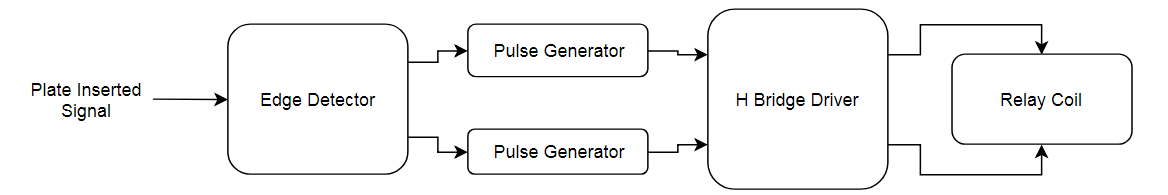
\includegraphics[width = \textwidth]{PR2Images/HBridgeCTRL_Block.PNG}
			\caption{Block Diagram depicting the control signals needed to drive the H bridge.}
			\label{fig:HBridgeCTRL_Block}
		\end{figure}

		The first implementation attempt first used a bidirectional edge detector circuit to generate the proper length pulse on any edge, followed by logic to determine the direction of the edge, such as in Figure \ref{fig:BidirectionalEdgeScheme}.  This required the use of an XOR gate in addition to typical NAND/NOR, and may be prone to race conditions resulting in both output signals going high at once.  For instance if C goes HIGH before D goes LOW, signal F and E could both asserted.  While this would not break the integrated H bridge solution, this is undesirable behavior, and the use of different types of gates would increase the cost and complexity of the BOM.

		\begin{figure}
			\centering
			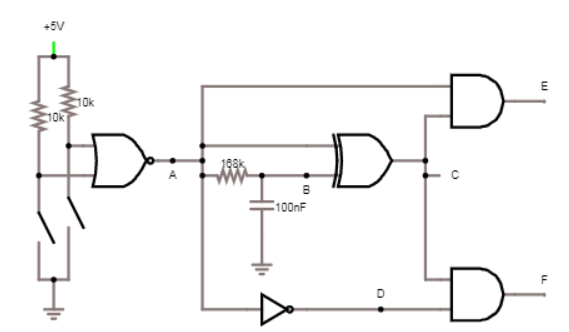
\includegraphics[width = 0.6\textwidth]{PR2Images/BidirectionalEdgeSchem.PNG}
			\caption{Edge detector and pulse generator.  This method first generate the necessary pulse on any edge, then extracts which edge (rising or falling) and sends the appropriate signal.}
			\label{fig:BidirectionalEdgeScheme}
		\end{figure}

		\begin{figure}
			\centering
			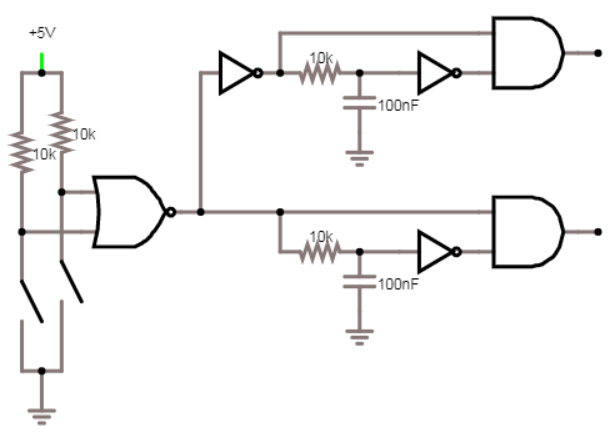
\includegraphics[width = 0.6\textwidth]{PR2Images/ParallelEdgeSchem.PNG}
			\caption{Edge detector and pulse generator.  This method applies one rising edge detector in parallel with one falling edge detector.  Note that the falling edge detector (top) is the just a rising edge detector with the input inverted.}
			\label{fig:RisingFallingParallel}
		\end{figure}

		\begin{figure}
			\centering
			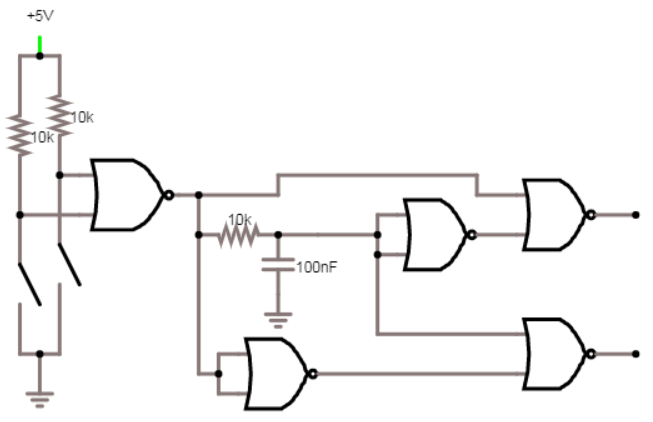
\includegraphics[width = 0.6\textwidth]{PR2Images/NOREdgeSchem.PNG}
			\caption{Edge detector and pulse generator.  This improved method combines the delay element of the previous one, and is implemented only with NOR gates, which helps with implementation.}
			\label{fig:ImprovedEdge}
		\end{figure}

		An alternative circuit is a rising edge detector in parallel with a falling edge detector, as shown in Figure \ref{fig:RisingFallingParallel}.  In this circuit, the signal is buffered then sent through an RC low pass filter to delay any edges and is inverted.  AND gates compare the delayed/inverted signal with the original and will output a pulse of proportional length to the RC constant of the filter if the two signals do not match.  This particular implementation would require 3 inverters, a buffer and two ANDs.  A simple optimization can combine the delay element into a single RC filter, which is fine if the pulse lengths for the two outputs can be the same length (in this case the requirement for both is $>$ 10 ms, so this is fine).  Figure \ref{fig:ImprovedEdge} demonstrates such a scheme.  In this implementation, the original signal, its delayed version, and their inverses are available to a pair of AND gates.  These inverters and gates should have Schmitt Trigger inputs to ensure a clean transition to generate the pulses.  With the signal labels from Figure \ref{fig:ImprovedEdge}, the function of the circuit can be reduced to a simple truth table

		\begin{center}
		\begin{tabular}{c c|c c}
			A & D & R & F \\
			\hline
			0 & 0 & 0 & 0 \\
			0 & 1 & 0 & 1 \\
			1 & 0 & 1 & 0 \\
			1 & 1 & 0 & 0
		\end{tabular}
		\end{center}

		This can be written as a set of boolean equations:

		\begin{align}
			R &= A \cdot \overline{D} \\
			F &= \overline{A} \cdot D
		\end{align}

		Because NOR/NAND gates are typically easier to implement and can also be used for the inverters, DeMorgan's Theorem can be used to convert these to their complimentary equivalents:

		\begin{align}
			R &= A \cdot \overline{D} = \overline{\overline{A} + D}\\
			F &= \overline{A} \cdot D = \overline{D + \overline{A}}
		\end{align}

		which can be implemented solely with NOR gates.  This is a perfect application of a quad, two input NOR gate such as the SN74HC7002 with Schmitt Trigger inputs \cite{SN74HC7002datasheet}.

		As the minimum pulse length to drive the relay is 10 ms, the pulse generate should aim for a longer pulse, perhaps 20 ms, to ensure the relay has been set to the correct position.  To determine the RC constant necessary to generate this pulse, consider the $V_{th}$ parameters of the SN74HC7002.  At $V_{CC} = 4.5V$, the positive going threshold voltage is at minimum 1.55 V \cite{SN74HC7002datasheet}, which is the case where the shortest pulse would be produced on a positive edge.  Solving the equation for RC capacitive charging gives

		\begin{align}
			RC &= \frac{-t}{\ln\left( 1 - \frac{V_{th}}{V} \right)} = \frac{-20ms}{\ln\left( 1 - \frac{1.55V}{5V} \right)} = 0.0539 s
		\end{align}

		so plugging in $C = 1 \mu F$ gives $R = 53.9 k\Omega$.  On the other hand, the maximum threshold voltage for a negative going transition is 2.54 V.  These $R, C$ values give a pulse time of 

		\begin{align}
			t  = - RC\ln\left( \frac{V_C}{V_0} \right) = -(53.9 k\Omega)(1 \mu F) \ln\left(\frac{2.54V}{5V} \right) = 36.5 ms
		\end{align}

		which is sufficient, though a slightly lower RC constant could reduce the excess pulse length.

		A full subsystem schematic of the receiver thus far is attached at the end of the document.  As implemented, the circuit uses 5 NOR gates, which poses a gate optimization problem, as this is just one more than a standard quad gate chip.  Unfortunately, the SN74HC7002, which is one of the only NOR gate ICs with a Schmitt Trigger input that will work with 5V, costs \$2.75 per chip.  To get around this cost, it would be possible to use an external Schmitt Trigger Inverter such as a 74AHCT14 type \cite{74HCT14datasheet}, which can be had for \$0.37 per chip, in conjunction with a non-Schmitt Trigger NOR gate, such as the 74AHCT02 \cite{74AHCT02datasheet}, which is just \$0.35 each.

		However, at this point, it may be cheaper and easier to use a microcontroller to perform this logic.  The obvious benefits of a microcontroller are:
		
		\begin{itemize}
			\item Reduced parts count: no need for external logic chips
			\item Can implement more complex logic, such as on board assurance that both H-bridge signals will not be on simultaneously
			\item Programmable debouncing of plate-detect pins
			\item Programmable pulse length for H-bridge driver
			\item Can also be used to control the adjustable power supply
		\end{itemize}

		Particularly because of the unknowns of the bounce characteristics of the pogo pins, the benefit of being able to easily adjust the debouncing is huge.

		To choose an appropriate microcontroller to determine if its cost will be worth it, the necessary features must be decided.  The first decision is how many receivers should be controlled by a single microcontroller.  The most straightforward replacement would be a one package per receiver.  This doesn't seem like the best option because any overhead required to implement the MCU would need to be repeated for each receiver.  The other extreme would be a single microcontroller for the entire main board.  This is not perfect either, as it would need a large number of GPIO, which is often supplied in difficult to assemble BGA type or other small packages.  In addition, a single centralized microcontroller would require long traces to reach the receivers, which could cause issues with signal integrity.  As the LV8548MC-AH are dual H-bridge drivers, a good compromise between these extremes is two receivers per microcontroller.  The microcontroller could be placed between two adjacent receivers to keep traces relatively short.

		To determine the number of GPIO required, count the number of I/O to this logic required per receiver:

		\begin{itemize}
			\item (2) Plate detect input pins
			\item (2) H-bridge driver outputs
			\item (2) Power Select outputs
			\item (2) Power Select inputs
		\end{itemize}

		This suggests a microcontroller with 16 GPIO is required for two receivers.  One cheap MCU available meeting this requirement is th ATTINY261A-MNR \cite{ATTINY261Adatasheet}, available in a 32-VQFN package for \$0.43.  A slightly larger package is the ATTINY40-SUR \cite{ATTINY40datasheet} in a 20-SOIC package for \$0.53.  The latter has 18 GPIO which could be useful for additional features later on, such as I2C communication between chips.  Although either of these or a number of others would work, the ATTINY40's extra GPIO package size make it a reasonable choice for this application, and actually reduces cost over the use of discrete logic components mentioned above.

		Now the function of the circuits described above can be implemented in code on the ATTINY40 and can be updated after fabrication.  A block diagram of the necessary functions is shown in Figure \ref{fig:MicroBlockDiagram}, along with a schematic showing the ATTINY40 interfacing with the peripherals at the end of the document.

		\begin{figure}
			\centering
			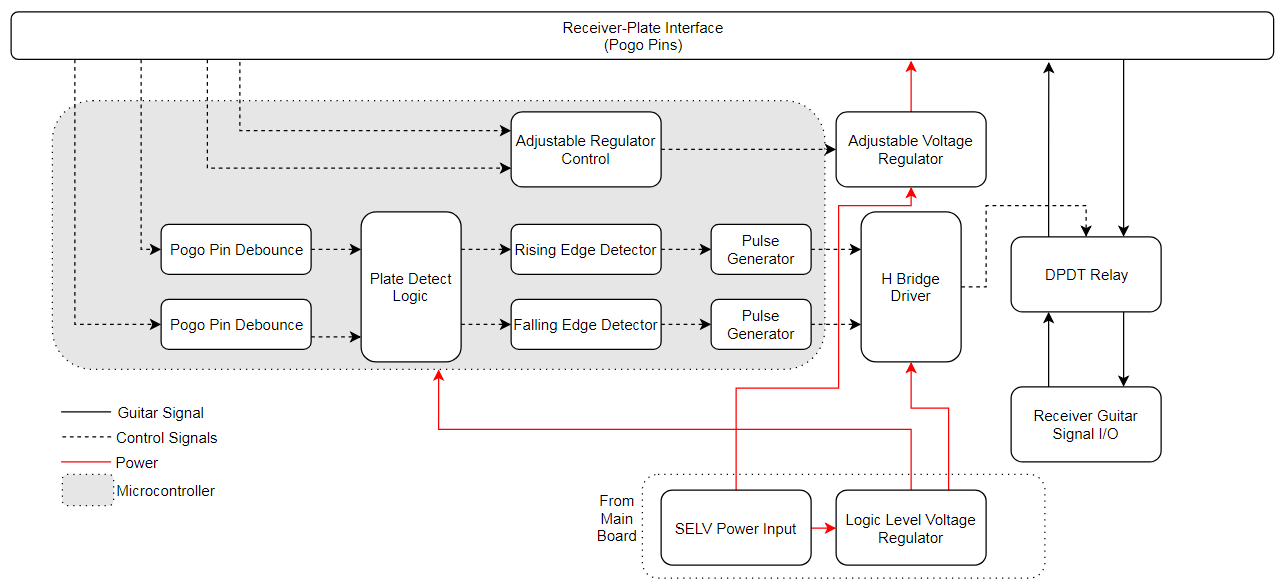
\includegraphics[width = \textwidth]{PR2Images/ReceiverBlockDiagramMCU.PNG}
			\caption{Receiver block diagram.  The blocks within the microcontroller are to be implemented in firmware.}
			\label{fig:MicroBlockDiagram}
		\end{figure}

		\subsubsection{Main Board Size, Routing, and User Interface}
		Stepping up in scale from the level of individual receivers to the entire solution system, the number and routing configurations of receivers is the next decision that needs to be made.  Though not of vital importance, the number of receivers will affect the number of pedals that can be tested at once, and the dimension of these receivers will affect the routing options available to the user.

		One of the biggest issues in this project is in the user interface.  The user interface should reflect the simplicity and tactile nature of the receiver-plate mating operation, where the user must only insert the pedal into the receiver to activate it.  However, this becomes difficult when the user is allowed to access many routing configurations.  The number of possible routing configurations for $n$ receivers quickly grows as $n$ increases.  This makes it difficult to display the current routing information to the user, let alone to allow the user to choose a different configuration.  Thus, an important design choice is striking a balance between sophistication and functional versus clarity, intuition, and ease of use.

		A method to simplify the routing is to layout the receivers in a grid, where the signal can move between rows at between every column.  The size of this grid should be informed by the likely scenarios that guitarists will test their pedals.  Though parallel routings can provide very interesting sounds, allowing only two rows for a maximum of two pedals in parallel at any point in the signal chain seems like a good space and complexity compromise.  This means that at any junction between rows and columns, the signal can either be kept in series within a row, or it can be split to an adjacent row.  Figure \ref{fig:JunctionRouting} shows the possible routing options: each arrow is a binary variable that can be chosen whether or not to allow signal to flow or not.

		\begin{figure}
			\centering
			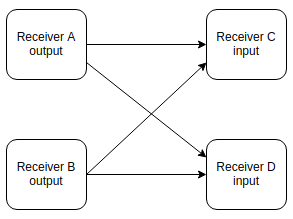
\includegraphics[width = 0.4 \textwidth]{PR2Images/JunctionRouting}
			\caption{Possible signal routings at a 2 x 2 junction.  Each of the arrows can be on or off, so there are $2^4$ possible combinations at this junction alone.}
			\label{fig:JunctionRouting}
		\end{figure}

		\begin{figure}
			\centering
			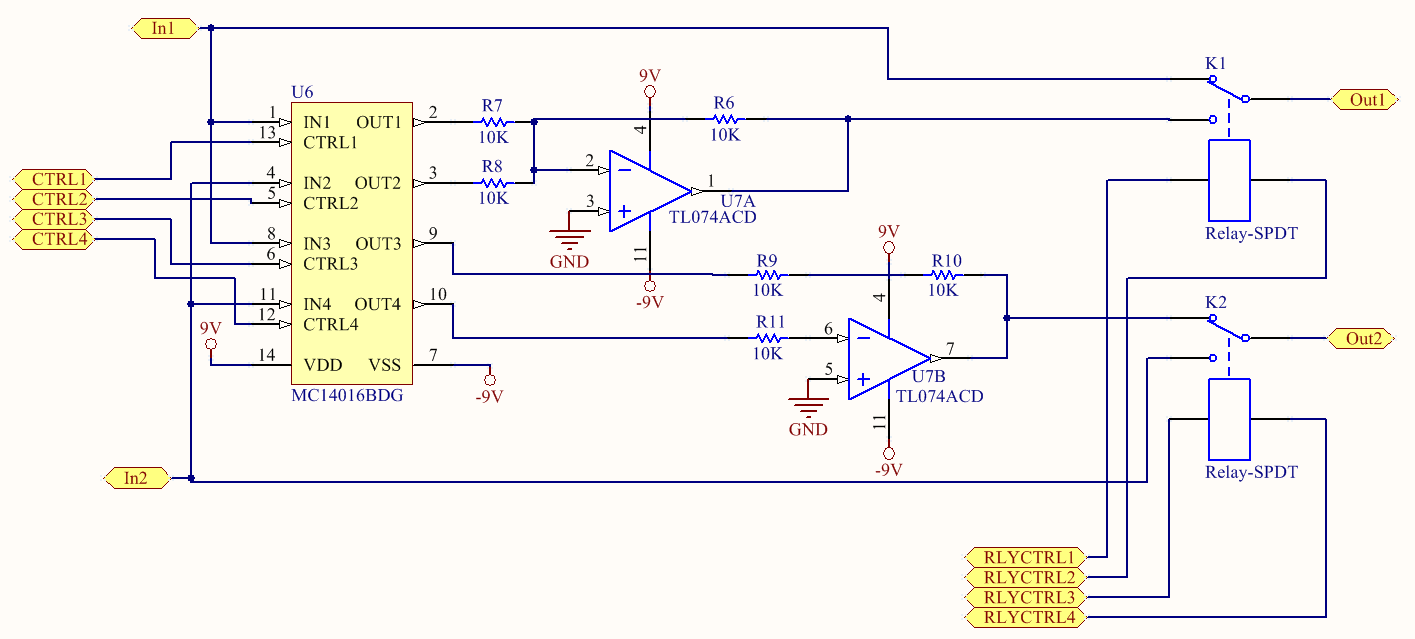
\includegraphics[width = \textwidth]{PR2Images/SignalJunctionSchematic.PNG}
			\caption{Implementation of signal routing at junctions.}
			\label{fig:JunctionSchematic}
		\end{figure}

		A specific implementation of one of these junctions should attempt where possible to use relays, for much the same reason that they were chosen for the receiver bypass mechanism.  Figure \ref{fig:JunctionSchematic} shows a circuit performing this function, where the switches and relays are control input signals.  When the signal is routed on the same row, it passes through a relay.  This is good for maintaining signal integrity.  However, when a signal changes rows, namely when a mono input is split or a pair of inputs is mixed, it will pass through some solid state switches.  This is acceptable because these operations require buffering or summing anyways.  Though the case where a signal changes rows but does not mix or split passes through unnecessary active components, this should not be a common configuration, and the added cost of using a relay for these switches is not justified.  The summing amplifier is an inverted variety, required another inverting buffer on the output.  It is possible that these inverting buffers could be externally controlled to allow for mixing of circuits that output signal at opposite polarity (perhaps because one of them inverted the signal), but that feature can be added later.  The relays need to be separate SPDT types rather than the same model used in the receiver bypass circuitry because they must be controlled separately.

		Guitarists typically have an intuitive understand of simple signal flow between pedals because with the visual clues of the cables that are used to make these connections.  An effective user interface would take inspiration from this, visually showing the connections between receivers.  One simple way of doing this is with lights that illuminate the signal path.  Edge-lit acrylic with surface engraving similar to the one in Figure \ref{fig:EdgeLitExample} could be used to provide a clean and consistent lighting.  This would work well with the junction routing discussed above because of its simplicity.

		\begin{figure}
			\centering
			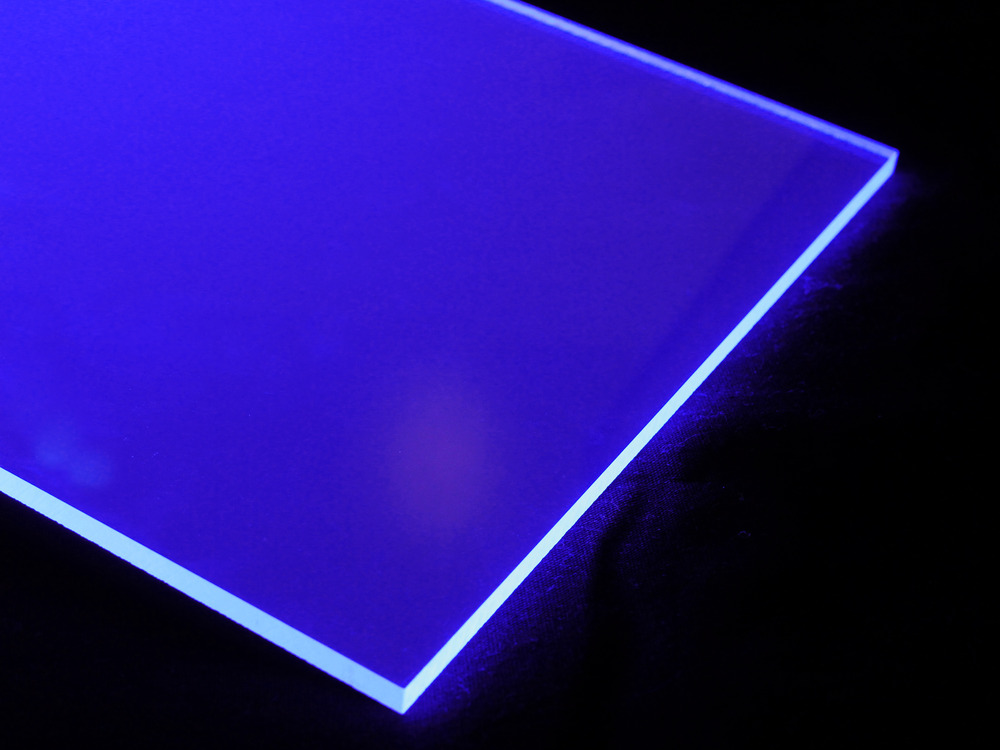
\includegraphics[width = 0.3\textwidth]{PR2Images/AcrylicEdge}
			\caption{One possible user interface for display the current routing state.  Designs may be rastered into the acrylic's surface as well.}
			\label{fig:EdgeLitExample}
		\end{figure}

		One simple method for the user interaction might be push buttons or tactile switches located near the signal paths being activated (the arrows in Figure \ref{fig:JunctionRouting}) such as the MJTP1230 \cite{MJTP1230datasheet} available for \$0.11 a piece.  This simple option would be very effective if it could be mounted underneath the acrylic light pipe mentioned above, in order to integrate the user's experience with the display and switch elements.  Because this interface will be part of the second prototype, there is still time to determine if this is possible.

		Another possible technique for user interaction could be capacitive touch sensors underneath the acrylic.  See \cite{CypressCapSense} for an explanation of capacitive touch sensing.  In essence, a cap touch sensor uses a sensor electrode on the circuit board, insulated by some overlay to form a parallel plate capacitor with a user's finger when it comes in close proximity to the electrode.  Using either the self or mutual capacitive sensing method, his capacitance is measured to determine if the sensor has been pressed.  In this particular application, the acrylic light diffuser could also be used as the insulating overlay for the sensor.  This would do a great job of combining the display and switch elements into a single unit for the user.  This technique requires a controller to operate the sensing mechanism, which could include a fully featured microcontroller such as the ATTINY40 previously discussed \cite{ATTINY40datasheet}, or a dedicated IC like the IQS127 from Azoteq \cite{IQS127datasheet}.  Some downsides associated with this technique are sharp signal edges at the sampling frequency of the sensor, which could potentially couple into the audio signal.  This should not be a major issue because this frequency is typically in the 100s of kHz \cite{IQS127datasheet}, which is far above the audio range.


\section{Prototyping Plan}
	As hinted at throughout the Design portion of this document, the prototyping for this project will take place in two main stages.  The first, to be completed this fall, will focus on the fabrication and testing of a single receiver board and associated plate.  Because the entire solution contains a number of instances of this subsystem and because the receiver subsystem is vital to the performance of the solution overall, its implementation should be ironed out before expanding scope to the routing interface.

	A block diagram of the system was shown in Figure \ref{fig:MicroBlockDiagram}.  A schematic of the electrical system is shown at the end of the document.  The components have been chosen in an attempt to make the board compatible with manufacturing on a PCB mill, such as the one in Maxwell Dworkin.  If the circuit board can be milled instead of produced by a fab-house, this will reduce the time and cost associated with prototyping these circuit boards.

	The second prototype will expand in scope to the full size product with multiple receivers and a complete user interface.  This will be where the routing implementation and interface will be tested.


\section{Measurements}
	In order to compare the performance of the prototype to the desired specifications, each metric must be measured.

	\subsection{Swapping Time}
	Measure the time required to swap one pedal for another.  As this is the simplest and most likely use scenario, and the swapping of a single pedal is the basis for all more complicated actions, this is a good metric for determining how much faster using the solution will be than the current method.  The experiment will start with a single pedal in series between the guitar and amplifier, with all necessary signal and power connections made.  The participant in the test plays the guitar through the pedal, validating that it the setup is functional.  On a signal, a timer starts while the guitarist stops playing, removes the current pedal from the signal chain, replaces it with the alternate pedal, which is readily on hand, and then tests that the new setup is functional by proceeding to play the guitar.  The timer stops once the participant begins playing again.

	It is important to use the same test procedure both when using the solution and when characterizing the typical method.  When testing the typical method, the guitarist must mute the amplifier to prevent popping, unplug signal and power from the pedal, plug in signal and power to the alternate pedal, then turn the amplifier on again.  When testing the solution system, the guitarist must lift the pedal plate out of the receiver, and insert the alternate pedal into the receiver.

	Because this test relies on a number of variables, including the person performing the test, it must be repeated multiple times per participant, with a number of different participants.  The participant should be told what steps need to be taken for a successful swap to be achieved in this test.

	Performing this test on the solution requires only one receiver unit, so this measurement can be taken as soon as the first prototype is complete.

	\subsection{Compatibility}

	Using the list of all pedals available at a particular retail store, count the number of pedals on this list than will work with this solution electrically and mechanically.  In particular, for a pedal to be considered compatible, it must

	\begin{itemize}
		\item Be powered by a supply voltage and current available from the solution
		\item Use a power connector supported by the solution
		\item Be fully functional with the I/O available through the solution (single input and output)
		\item Have screw holes on the bottom plate that align for proper use with the plate mounting system
		\item Not be effected operationally by use of this solution
	\end{itemize} 

	If a pedal fits these criteria, it can be considered compatible with the solution.  The percentage of compatible pedals is the ratio of compatible pedals to the total number of pedals tested against these criteria.

	While this test could be performed with physical pedals, it would be difficult to access enough to be statistically significant.  Thus, this measurement can be performed by comparing the specifications of the list of pedals available at the Guitar Center retail location to the capabilities of the solution.  Physical testing should be performed as an auxiliary to this.

	\subsection{Cost}

	In general, the cost should represent the cost for constructing a single unit of the solution, rather than price it would sell for, as the latter is too heavily affected by external factors.  However, the cost to produce a unit can be estimated by the sum of the material costs plus the estimated labor cost.  This will of course scale with volume, so an estimated volume should be on the order of the number of guitar retail stores in the United States, about 500.

	\subsection{Signal to Noise Ratio}
	$SNR = 20 \log \big( \frac{A_{signal}}{A_{noise}} \big)$.  When testing the unit, measure signal with sinusoid signal at varying frequencies in desired range (DC, 20Hz, 200Hz, 2kHz, 20kHz), as well as pink noise.  This measurement can be taken with an Audio Precision measurement device.

	Initial tests can be made with the first prototype, though because of its simple signal routing through a relay, the performance should be very good.  A more telling test will be of the second prototype when the signal must pass both through the bypass relays as well as the routing circuits.

	\subsection{Frequency Response}
	The frequency response can be measured with the FFT function of an oscilloscope.  Input a sine wave swept from DC to 100 kHz and compare the ratio of the output to the input.  This test can also be performed with an Audio Precision measurement device.

	Like the previous test, initial measurements can be made with the first prototype, though because of its simple signal routing through a relay, the performance should be very good.  A more telling test will be of the second prototype when the signal must pass both through the bypass relays as well as the routing circuits.

	\subsection{Switching Speed}
	Using an oscilloscope, measure the time difference between the detection of plate insertion and the relay switch settling on the desired output.  To determine the beginning of this period, look at the connection of the mate-last break-first pogo pins used to detect if the plate has been inserted or is being removed.  Determining the end of this period requires looking at the output signal.  To get a visual on when the output changes, connect the input of the system (the guitar end) to ground, and use a "pedal" whose output is always a known voltage, for example 5V.  The output will show a transition from 0V to 5V at the output when the plate containing this "pedal" is inserted.

	This can be measured on the first prototype.

	\subsection{Transient}
	The transient on the output signal due to switching can be due to a number of causes.  First, there may be an instantaneous difference between the input/bypass signal and the effected signal returning from the pedal.  One example of this might be a pedal that inverts the signal.  In addition, many pedals use a single supply voltage and have their amplifiers biased to Vcc/2, the leakage current through the decoupling capacitors on the input and output can cause nonzero voltages on the output if pull down resistors are not used, again leading to an instantaneous change in voltage level \cite{OrmanBypassMeasurements}.

	Because these transients will occur differently each time, this must be tested with a variety of effects and in many trials.  Because the transients will have a strong high frequency component that will be very distinct from the typical signal, it should be easiest to detect them in the frequency domain.  To standardize the test and ease measurements, use a 1 kHz sine input and measure the power of any transients in the frequency domain, and compare to the standard power of the sine wave.  Perform with different pedals at different frequencies (100 Hz, 1 kHz, 10 kHz).

	The Audio Precision measurement device can also perform click and pop transient measurements \cite{APclickpopmeasurement}.  This measurement can be performed on the first prototype as well.

	\subsection{Intuition}
	This idea behind this specification is a good design guideline, but it is hard to determine the best way to quantify this.  A user manual will certainly be one of the products of this project, so a word count is one easy method.  This is an area that could use some suggestions!

	\subsection{SELV Compliance}
	This should be evident from the design.  However, one test might be to verify that all signals in the device are below 60 VDC, which can be performed with a multimeter.

\section{Analysis}
	For some of the specifications, it is easy to determine if the measurements satisfy the requirements.  For instance, the System and Incremental Cost are related simply to the materials and manufacturing cost required to contruct the prototype (not including NRE costs).  Similarly, SELV compliance guides the design, so this will be satisfied after a confirmation that no high voltages are present in the unit.

	A number of the specifications relate to characterizing the signal, including the SNR, Frequency Response, and Transient metrics.  For each of these, a one sample, one-sided t-test should be used to determine if their value meets or exceeds the specificed requirements.  The transient response can also follow this procedure.  The t-test should be performed for both the minimum and the ideal value of each specification.  For these specifications, each measurement be performed 10 times to begin with, with aspirations of achieving a significance level of 0.05.  In each case, the null hypothesis is that the prototype does not acheive the specified performance, while the alternative is that the prototype does exceed the specified performance.

	The results of these tests can be displayed in bar graph with error form, which will show comparisons between prototypes once iterations have been made.  These plots can also show with a horizontal line the desired specifications.

	The compatibility measurement, can be performed in a similar manner to the above, though it will have a much larger sample size.  An interesting and useful analysis will be to determine common features of pedals that are not compatible with the prototype.  This can be used to aid in the design of subsequent iterations to improve this metric.

	Finally, the main metric to be tested is the swap time.  Unlike the specifications thus far, this data will be a paired, by test subject, so a paired, one-sided t-test should be used.  Beacuse this specification compares measurements from the current method and the solution, and it is likely that different users will have variations in the time it takes to swap pedals, a paired-data one-sided t-test should be used.  Because of sample to sample variations by a single test subject, each should perform the test several times for both the normal method and the solution method.  Several test subjects may be used.  This data can be visualized with a grouped bar graph with error/deviation bars.  One group will be the average time for the standard method and the other will be the average time for the improved method.  The independent variable would then be the test participant.  This would show trends that each test subject experienced.


\section{Logistics}

	\subsection{Updated Schedule}

	Note: \colorbox{green}{Green text} indicates complete work.  \colorbox{yellow}{Yellow text} indicates work in progress.  \colorbox{red}{Red text} indicates items that are behind schedule.

	The schedule up to weeks 7 and 8 has been updated by color to reflect state of completion.  The subsequent time line has been adjusted according to the current state and schedule.

	\begin{table}[H]
	\begin{tabular}{llp{4in}}
	Weeks    & Dates         & Plan \\
	\hline
	1 \& 2   & 9/2 - 9/15    &  \colorbox{green}{Complete and revise Project Proposal and meet with advisers}      \\
	3 \& 4   & 9/16 - 9/29   &  \colorbox{green}{Conduct experiments described above to help refine specifications.}  \color{green}Begin higher level block diagrams of system.  Progress Report \#1 due 9/28 \color{black}    \\
	5 \& 6   & 9/30 - 10/13  &  \color{green}Begin prototyping key features, such as pedalboard - plate interface. Rapid prototyping of features such as plate design to inform first prototype. Develop lower level block diagrams and begin schematic design. \color{black}    \\
	7 \& 8   & 10/14 - 10/27 &  \color{yellow}Electronic and Mechanical CAD design for first prototype.  The first prototype will be a single slot for testing the 1) reliability of electrical connections between plate and board, 2) mechanisms for attaching pedal to plate (mechanical and electrical), 3) strength of magnets needed to hold plate to board, 4) method for hot-swappable bypassing (sensing and actuation) \color{black}    \\
	9 \& 10  & 10/28 - 11/10 & Complete ECAD and MCAD design of single receiver prototype.  Progress Report \#2 due 11/5    \\
	11 \& 12 & 11/11 - 11/24 &  Begin fabrication of PCB, mechanicals.  Write code for receiver microcontroller.  In parallel, begin schematic design for full scale Prototype 2.  \\
	13 \& 14 & 11/25 - 12/8  &  Fabricate mechanical parts.  Assemble circuit boards.  Perform preliminary testing on first prototype.      \\
	15 \& 16 & 12/9 - 12/22  &  Continue testing and analyze results.  Outline goals/changes for next iteration.  Oral Design Review/Presentation 12/10    \\
	17 \& 18 & 12/23 - 1/5   &  Winter Break: Expect Little Progress    \\
	19 \& 20 & 1/6 - 1/19    &  Complete ECAD and MCAD for full scale prototype.  Write firmware for Work on firmware necessary for controlling routing.  Examine which UI interactions are most feasible (capacitive touch, tactile switches) \\
	21 \& 22 & 1/20 - 2/2    &  Return to campus.  Begin fabrication of prototype 2.     \\
	23 \& 24 & 2/3 - 2/16    &  Complete fabrication and perform full range of tests with analysis.  Progress Report \#3 due 2/15    \\
	25 \& 26 & 2/17 - 3/2    &  Update design with iterated improvements.    \\
	27 \& 28 & 3/3 - 3/16    &  Fabricate iterated design, test, and analyze. Begin outlines for Final Report.  Progress Report \#4 due 3/5   \\
	28 \& 29 & 3/17 - 3/30   &  Prepare for presentation.  Write final report, make last minute changes.  Final Oral Presentation 3/25  \\
	30 \& 31 & 3/31 - 4/13   &  Revise final report.  Final Written Report due 4/5    
	\end{tabular}
	\end{table}

	All schedule items between week 7 and week 23 have been shifted back to reflect the better clarity that is now understood compared to the first progress report.  Because the prototypes will progress in scope, this means that the full system prototype will not come together until after winter break.  As much design work as possible must be done over that time to ensure completion.

	\section{Updated Budget}

	\color{gray}
	Like the schedule, the budget is becoming more clear than the one from the project proposal.  One piece of feedback I received from a number of people is the lack of representation in my budget for acquiring guitar pedals for testing and design purposes.  Some possible sources of pedals might be from my own personal collection, from a collection held by the Music Department, and by interested Harvard affiliates and professors.  Purchasing pedals for this project seems to be an unnecessary expense, so I will avoid purchasing new units if possible.  
	\color{black}

	The cost of the solution will be related to the cost of its individual subsystems.  So far, the cost of each receiver subsystem is about:

	\begin{table}[H]
	\begin{tabular}{l l l|l}
	Component Type & Quantity & Unit Cost & Total\\
	\hline
	Capacitors & 7 & \$0.10 & \$0.70 \\
	Resistors & 5 & \$0.10 & \$0.50 \\
	Pogo Pins & 10 & \$0.66 & \$6.60 \\
	ATTINY40 & 1 & \$0.53 & \$0.53 \\
	MOSFETS & 2 & \$0.15 & \$0.30 \\
	LV8548MC-D & 1 & \$1.33 & \$1.33 \\
	LM317 & 1 & \$0.67 & \$0.67 \\
	LM7905 & 1 & \$1.50 & \$1.50 \\
	EA2-5SNJ & 1 & \$1.78 & \$1.78 \\
	\hline
	 & & & $\approx$ \$14
	 \end{tabular}
	 \end{table}

	 This does not include some of the one time costs such as input and output jacks for the entire system.  The exact cost can be determined once the BOM is complete.  Adding in the cost for manufacturing the mechanicals, a rough estimate of \$25 per receiver is reasonable.  Though the design of the junction signal routers is not yet complete, its cost is likely about half that of each receiver because it does not include the expensive pogo pins, though it will use a relay, relay driver, and microcontroller like the receiver.  There will be similar mechanical cost associated with the routers because of the user interface considerations.  So assuming \$25 per plate and \$20 per junction for 6 plates plus 4 junctions gives an estimate of \$180.  This is narrowly in the minimum goal price criteria, and with an assumption of another \$25 - \$50 of axillary mechanical costs, the cost will be close to the desired budget (though the ES100 budget of \$500 should cover the construction).  Using the PCB mill to fabricate the PCBs is a good way to save manufacturing cost for these prototypes.


\newpage
\bibliographystyle{plain}
\bibliography{ThesisSources}

\section{Appendix}
The first schematic is the discrete H bridge and IC logic implementation.
The second schematic is the microcontroller and integrated H bridge driver implementation that will be pursued for the first prototype.


\end{document}
